\documentclass[11pt]{report}
\usepackage{amssymb,amsmath}

%% enable markdown's stars to bold/italic sections of code -- requires lualatex!
\usepackage{luacode,luatexbase}
\begin{luacode}
   -- Use Lua captures to extract material affected by markdown
   function allstars (line) 
      line = string.gsub( line, "(%*%*%*)(.-)(%*%*%*)", "{\\bfseries\\itshape %2}")
      line = string.gsub( line, "(%*%*)(.-)(%*%*)", "{\\bfseries %2}" )
      line = string.gsub( line, "(%*)(.-)(%*)", "{\\itshape %2}" )
      return line
   end
\end{luacode}

\newcommand\markdownon{%
   \directlua{luatexbase.add_to_callback( "process_input_buffer", allstars, "allstars" )}}
\newcommand\markdownoff{%
   \directlua{luatexbase.remove_from_callback( "process_input_buffer", "allstars" )}}



%\usepackage[style=authoryear]{biblatex}
\usepackage[style=numeric]{biblatex}
\addbibresource{biblio.bib}
\addbibresource{my-publications.bib}
\addbibresource{mutual-modelling.bib}

\usepackage{pdflscape}

\usepackage{fontspec}
\defaultfontfeatures{Ligatures=TeX,Scale=MatchLowercase}
\setmainfont[]{cantarell}

\usepackage{graphicx}
\usepackage{wrapfig}
\usepackage{hyperref}
\urlstyle{same}  % don't use monospace font for urls
\usepackage[margin=4pt]{subcaption}

\usepackage[a4paper,left=2cm,right=2cm,top=1.5cm,bottom=1.5cm]{geometry}
\usepackage{longtable,booktabs}

\usepackage{pgfgantt}
\usepackage{rotating}

\usepackage{tocloft}

\usepackage{titlesec, blindtext, color}
\definecolor{gray75}{gray}{0.75}
\newcommand{\hsp}{\hspace{20pt}}
\titleformat{\chapter}[hang]{\LARGE\bfseries}{\hsp\textcolor{gray75}{|}\hsp}{0pt}{\LARGE\bfseries}


\renewcommand{\thesubsubsection}{}

\usepackage{xspace}
\newcommand{\project}{WizUs\xspace}

\newcommand{\task}[2]{\vspace{0.5cm}\noindent\emph{Task T#1}: {\bf #2}\par}

\newcommand{\D}[3]{\emph{Deliverable D#1} (M#2): #3\\}

\newcommand{\TODO}[1]{{\color{red}\textbf{TODO: #1}}}

\newcommand{\severin}[1]{{\color{red}\textbf{Severin: #1}}}
\newcommand{\toseverin}[1]{{\color{red}\textbf{To Severin: #1}}}
\newcommand{\eu}[1]{{\color{teal}\textbf{Guidelines EU ERC: #1}}}
\newcommand{\cellgrey}{\cellcolor[gray]{0.85}}

\setcounter{secnumdepth}{0} % prevent section numbering, but still add sections to ToC

\title{\project - Part B}

\begin{document}
\markdownon
\maketitle

\begin{center}
    ERC Consolidator Grant 2020

    \vspace{2cm}
    \textbf{\LARGE Socially-Driven Robots to Support Human-Human Interactions}

    \vspace{2cm}
    {\Huge \project}

\end{center}

    \vspace{2cm}

\begin{itemize}
    \item Principal Investigator: \textbf{Dr Séverin Lemaignan}
    \item Host institution: \textbf{University of the West of England, Bristol Robotics
        Laboratory}
    \item Duration: \textbf{60 months} (5 years)
\end{itemize}

\section*{Abstract}\label{abstract}

\eu{The abstract (summary) should, at a glance, provide the reader with a clear
understanding of the objectives of the research proposal and how they will be
achieved. The abstract will be used as the short description of your research
proposal in the evaluation process and in communications to contact in
particular the potential remote referees and/or inform the Commission and/or the
programme management committees and/or relevant national funding agencies
(provided you give permission to do so where requested in the online proposal
submission forms, section 1). It must therefore be short and precise and should
not contain confidential information. \\
Please use plain typed text, avoiding formulae and other special characters. The
abstract must be written in English. There is a limit of 2000 characters (spaces
and line breaks included).}

The \project project investigates how socially-driven robots can have a lasting, 
positive impact on the society. It defines the concept of \emph{robot-supported
human-human interactions} as a general framework to study and implement 
socially-aware intelligent robots, able to foster rich and positive interactions
between people.

Grounded in the psycho-social literature of human cognition, the project delivers
major conceptual, technical and experimental contributions to the field of AI, 
with a special focus on having ethical safeguarding mechanisms built-in 'by 
design' into the robot.

Doing so entails conceptual and technological breakthroughs, as well as a research
methodology that puts the end-user needs at the centre of the design process. 
Building on a range of multidisciplinary techniques, including novel interactive 
machine learning techniques, \project paves the way for a better understanding of 
the societal challenges raised by the rapid development of AI and robotics.

\newpage

\tableofcontents

\pagebreak

%%%%%%%%%%%%%%%%%%%%%%%%%%%%%%%%%%%%%%%%%%%%%%%%%%%%%%%%%%%%%%%%%%%%%%%%%%%%%%%%%%%%%%%%
%%%%%%%%%%%%%%%%%%%%%%%%%%%%%%%%%%%%%%%%%%%%%%%%%%%%%%%%%%%%%%%%%%%%%%%%%%%%%%%%%%%%%%%%
%%%%%%%%%%%%%%%%%%%%%%%%%%%%%%%%%%%%%%%%%%%%%%%%%%%%%%%%%%%%%%%%%%%%%%%%%%%%%%%%%%%%%%%%
%% Names of the Work packages

\newcommand{\wpOne}{Project management \& dissemination}
\newcommand{\wpOneShort}{\wpOne{}}

\newcommand{\wpTwo}{Framing robot-supported human-human interaction}
\newcommand{\wpTwoShort}{Framing r-HHI}


\newcommand{\wpThree}{Ethical-by-design socio-cognitive architecture for robot-supported human-human interactions}
\newcommand{\wpThreeShort}{Socio-cognitive architecture}

\newcommand{\wpFour}{Social situation assessment}
\newcommand{\wpFourShort}{\wpFour{}}

\newcommand{\wpFive}{Data-driven social behaviour generation}
\newcommand{\wpFiveShort}{Social behaviours}

\newcommand{\wpSix}{Study 1: social companion at the hospital}
\newcommand{\wpSixShort}{Hospital study}

\newcommand{\wpSeven}{Study 2: robot-supported SEN chools}
\newcommand{\wpSevenShort}{SEN schools study}




%%%%%%%%%%%%%%%%%%%%%%%%%%%%%%%%%%%%%%%%%%%%%%%%%%%%%%%%%%%%%%%%%%%%%%%%%%%%%%%%%%%%%%%

\newrefsection

\chapter{B1.a. Extended Synopsis of the scientific proposal}\label{part1}
\eu{(max 5 pages)}

\eu{The Extended Synopsis should give a concise presentation of the scientific
proposal, with particular attention to the ground-breaking nature of the
research project and the feasibility of the outlined scientific approach.
Describe the proposed work in the context of the state of the art of the field.
References to literature should also be included. References do not count
towards the page limits. It is important that this extended synopsis contains
all essential information including the feasibility of the scientific proposal
since the panel will only evaluate Part B1 at step 1.}

\TODO{why is it groundbreaking?}

\TODO{impact/outcomes?}

\TODO{discuss r-HHI more: what does it really mean to use a robot to support
HHI? link to responsible AI?}

\TODO{make sure everything in B1 is strongly grounded in litt}

\section{Long-term vision and targeted breakthrough towards that vision}

To assert and reinforce an European \textbf{leadership in AI and robotics that
is socially responsible} and guarantees, \textbf{by design, long-term benefits
to the society}, a strong vision, combined with unique scientific leadership, is
essential.  \textbf{\project aims at building this capacity}. \project is about
developing and integrating \textbf{beyond-state-of-art socio-cognitive
capabilities} in service and companion robots, while researching, defining and
implementing the \textbf{conceptual framework that we need for a trustworthy and
responsible AI}: \project will realise \textbf{a vision of AI and social
robotics that places the human at the centre of the technology; supports
stronger, more cohesive social interactions; empowers rather than isolates}.
This objective is underpinned by the key concept of \textbf{robot-supported
human-human interactions}, which conceptually reverses the traditional, technology-centric,
views of human-robot interactions.




\subsection{The case for robot-supported human-human interactions}

Indeed, in a time where robots are on the verge of becoming pervasive in our
daily human environment, can we ensure 'by design' that robots are to become
powerful tools to support more and better, positive interactions \emph{between
the people themselves}, and build a stronger, more cohesive society? Beyond
Human-Computer Interaction (HCI) and Human-Robot Interaction (HRI), \project is
a forward-looking, ground-breaking project that aims at establishing
\textbf{Robot-supported Human-Human Interactions (r-HHI)} as the next step
toward a Responsible AI: \textbf{the scientific investigation of how social
robots can create, shape and support strong, sustained, positive
\emph{human-human} relationships}.

As a researcher who has been working for the last 12 years in the field of
human-robot interaction (and child-robot interaction in particular), I have been
a direct witness -- through being one of the architects -- of the crossing of a
critical milestone: the emergence of \textbf{long-term social interactions}
between robots and humans. Over the last two
years in particular, we observe an explosion of the number of studies involving
social robots, deployed in real-world settings (schools, care centres) over
relatively long periods of time (up to 2 or 3 months at a time). Even though
these robots are rarely fully autonomous, they do already show high levels of
autonomy~\cite{emmanuel}, with full autonomy in sight~\cite{strands}.\TODO{litt review}

While many see these developments positively,
others express skepticism or worry that this technology might lead to a
dehumanisation of our society. Indeed, if artificial agents are to engage into
social interactions with us, and enter what many view as a form of a 'private
domain', reserved to humans, pressing ethical questions need to be answered:

\begin{itemize}
    \item how to ensure that social robots are not used to simply replace the human
        workforce to cut costs?
    \item can we guarantee that the use of social robots will always be ethically motivated?
    \item even further, can we implement some ethical safeguarding at the core
        of the system (like an ethical \emph{black-box}~\cite{winfield})?
    \item what about privacy? how to trust that robots in our home or school or
        hospital will not eavesdrop on our private lives, and, in the worst
        case, will not be used \emph{against} us?
\end{itemize}

These questions are not only legitimate, but also pressing, and the EU ought to
be at the forefront of that research. The recent rise of
personal assistants like Amazon Alexa or Google Home, with the major privacy concerns
that accompanies their deployments in people home, shows that letting the
industry set the agenda on these questions is not wise -- and robots can
potentially be much more intrusive than non-mobile smart speakers.

Social robots have two unique properties which distinguish them from these smart
speakers, and significantly complexify their conceptual framing. First, they are
fully embodied, and they physically interact with their environment, from moving
around, to picking up objects, to looking at you; second, willingly or not, they
are ascribed \emph{agency} by people.  This second difference has far-reaching
consequences, from affective bonding to over-trust, to over-disclosure of
personnal, possibly sensitive, informations \TODO{cite paper HRI children
disclosure}.

Due to the complex interplay between the technical implementation, the
socio-psychological determinants of the interactions, and the multiple ethical
mechanisms that have to be built-in the system, it is difficult to build one
coherent and consistent perspective on the whole question. Indeed, the
conceptual, intellectual framework emcompassing both the internal cognitive
mechanisms required by socially intelligent robots, as well as their role and
impact in the society, only exists in fragmented, disconnected pieces.


The lack of such a proper conceptual framing is a critical issue: for robots to
have a positive impact on the society, with strict ethical and privacy-related
safeguarding, it is urgent that the wider academic and intellectual communities,
beyond technologists, embrace this question and build up the debate on the
acceptability of robots in our society. And \textbf{this also calls for a major
re-thinking of the traditional paradigm of Human-Robot Interaction}.
Tradionally, individual cognitive functions (like natural language processing,
emotion recognition, proxemics-aware navigation) are implemented in robots, with
the ill-supported assumption that 'the more available functions, the more
socially-capable the robot'. This assumption is questionable, and, at any rate,
does not address the 'why': why does it decides to do what it does? What drives
the behaviour of the robot? The case for \emph{teleological} (ie goal-driven)
robotic architecture has been made in the past~\cite{oudeyer}, but only
effectively realised for relatively simple cognitive systems (like
curiosity-driven robot animals~\cite{oudeyer,isir} or motor babbling in
infant-like robots~\cite{cangelosi,iit}). However, socially-driven robots,
participating in complex interactions with humans, have been barely
investigated~\cite{needacite}.

\textbf{Being socially-driven to do 'good' is however essential in ensuring
trustworthy, socially responsible robots}. Nutrured by decades of research in
understanding human social cognition and its social motivations, one of the key
deliverables of \project is \textbf{inventing and building a
principled and socially-driven cognitive architecture} for tomorrow's social
robots. This socially-driven, teleological architecture, intrinsically designed to
\textbf{support stronger, positive human-human interactions} is what underpins
the concept of \emph{robot-supported human-human interactions}.

\project aims at building unique European capacity to assert leadership in this
domain, and, beyond the specific deliverables of this 5-years project,
establishing the PI as a world-leader in goal-driven, socially-responsible
robotics.

\subsection{The \project vision}


'Socially intelligent' robots require unique, beyond state-of-the-art,
capabilities to \emph{(1)} understand the social interactions (social
situation awareness), \emph{(2)} autonomously decide the best course of action for
short-term and longer-term social influence, and \emph{(3)} perform the
appropriate social actions and exert appropriate, responsible social influence.

However, extreme complexity hides behind these seemingly well-delineated steps:
not only the required technology is itself beyond state-of-the-art, but the
interplay between technology, socio-cognitive psychology, privacy and ethics is
only starting to be researched and understood. Together, it forms what is called
a \emph{wicked problem}~\cite{tonkinwise2015design} -- a problem whose social complexity
means that it has no determinable stopping point. \textbf{\project offers an
strong vision and an ambitious, evidenced-based, methodology to significantly
advance our understanding of this problem}.

Over the course of 5 years, I will specifically investigate the following
research questions:

\begin{itemize}
    \item \textbf{R1} [conceptual level]: what are the adequate social 'boundaries' that the robot need to
        account for, to realise social utility while ensuring social
        responsability?
    \item \textbf{R2} [technology level]: where are the technological gaps in the artificial social cognition
        capabilities required to effectively act inside of these social
        boundaries? how to fill them?
    \item \textbf{R3} [conceptual \& technology level]: what are the principles underpinning a
        socially-driven teleological architecture, leading \emph{by design} to a
        responsible, trustworthy, human-centered robot behaviour, supportive of human-human
        interaction? how to realise such a system?
    \item \textbf{R4} [experimental level]: can we demonstrate in complex, real
        world conditions, the effectiveness and usefulness of the robot-supported human-human
        interaction paradigm?
\end{itemize}


\section{Implementation}

\subsection{Work programme}

Indeed, the \project vision unfolds along four main axes, reflected in the
structure of the workpackages: \textbf{WP2} is dedicated to the conceptual
framing of the project (R1); \textbf{WP3} grows from WP2 to transpose the
conceptual framework into a principled cognitive architecture (R3); \textbf{WP4}
and \textbf{WP5} look at the technological underpinnings of this architecture
(R2); and \textbf{WP6} and \textbf{WP7} introduce two ambitious real-world
demonstrators of the \project approach (R4).

In addition, \textbf{WP1} is dedicated to the project management and the
supervision of the dissemination activities planned in the project.

\paragraph{WP1: \textbf{\wpOne}} (covers the duration of the whole project).
This workpackage encompasses

\TODO{complete this section}

\paragraph{WP2: \textbf{\wpTwo}} (Y1-3)

The basic ambition of \project is to create a conceptual framework
around social robots in the human society, by re-framing the widely accepted, yet
sorely unspecific, idea of \emph{human-robot interaction} into the more specific
idea of \emph{robot-supported human-human interactions}: the robot is considered
from the perspective of how it can \emph{support} humans, and in particular,
support stronger, positive interactions between humans. WP2's purpose is to research
and define such a framework that will
provide the (currently missing) conceptual frame around questions like: what role
for social robots? where to set the boundaries of artificial social
interactions? what does 'ethical-by-design', 'responsible-by-design' might mean
in the context of social human-robot interactions? 


\paragraph{WP3: \textbf{\wpThree}} (Y2-5)

\TODO{complete section architecture}

\begin{itemize}
    \item Intrinsic social motivation: do good
    \item bottom-up grounding for situation assessment and social situation
        assessment
    \item symbolic grounding of both environment and social situation using
        'human in the loop' OR data-driven symbolic grounding
    \item knowledge representation and symbolic reasoning for dialogue
        grounding, goal planning, knowledge exchange and linked data
    \item action execution using human-in-the-loop ML
\end{itemize}

\paragraph{WP4: \textbf{\wpFour}} (Y1-4)

In WP4, the project addresses the key scientific and technical underpinnings
required to effectively implement WP3's architecture:  the scientific
understanding and formalisation of the \emph{social fabric} in which the robot
is embedded, in its full complexity: spatial characteristics (proxemics; group
dynamics, complex, dynamic attentional mechanisms); psycho-social
characteristics (social roles and hierarchies; social groups; mental modelling;
anthropomorphic ascriptions); temporal characteristics (effects of novelty,
dynamics of anthropomorphism and mental ascriptions, shifting group dynamics).
This work will result in the formulation of a socio-cognitive model of the
social environment of the robot and the effective implementation of the model,
including the development of a complete social assessment pipeline, from social
signal perception (like automatic attention tracking, face recognition, sound
localisation, etc.) to higher-level socio-cognitive constructs, including group
dynamics and theory of mind. As detailled in Section B2, this will rely on
hybrid AI techniques, including symbolic (ontologies and first-order logic),
sub-symbolic (neural nets) and hybrid (conceptors) modelling.

\paragraph{WP5: \textbf{\wpFive}} (Y1-4)

Mirroring WP4, WP5 addresses the question of social behaviour \emph{generation}.
Indeed, designing behaviours that enable sustained, long-term engagement in a
social human-robot interaction is essentially an open research question. Three
main approaches to social behaviours generation exist today:
\emph{user-induced}, where the end-user interacts with the robot and ascribes
(knowingly or not) complex behaviours to the machine, while in reality the
robot's behaviours are simple and non-goal oriented (eg generating a noise or a
small movement when being touched). This has been used to great effect in
therapy robots, for instance (eg Paro). \emph{Off-the-shelf behaviours}, where
the robot relies on a set library of behaviours (that might be individually
relatively complex). The approach can elicit a strong initial social response
from the user, but this social response tends to vanish rapidly once the
'tricks' of the robot have been all discovered and become repetitive.  Besides,
as the robot does not typically maintain a long-term socio-cognitive plan of the
interaction, the behaviours are typically perceived as fun, yet pointless. This
is often observed in toy-like robots (eg Vector, Dot \& Dash). Finally, many
social robots avoid altogether the problem of generating behaviours by simply
offering to the end-user control over \emph{low-level behaviours} (eg, control
of the joints of the robot). This means that, even when the robot has relatively
powerful social perception capabilities (like recognising people and voice), no
real social behaviours is generated.

None of these three approach is satisfactory, and indeed, no approach to date
has been able to engage human users in long-term, sustained interactions.
\project aims at significantly advancing the state of the art in this regard, by
combining two emerging techniques: (1) a new data-driven, continuous approach to
behaviour generation inspired by Learning from
Demonstration~\cite{citationneeded}; (2) interactive machine learning in
high-dimensional input/output spaces~\cite{senft2020woz}, where I have shown
with my students promising results for generating complex social
behaviours~\cite{senft2019teaching, winkle2020coach} that fully involve the
end-users~\cite{winkle2020methodology}. By combining the two, \textbf{I target a
breakthrough in robots' social behaviours generation: the generation of
non-repetitive, socially congruent and transparent social
behaviours} (including gestures and gazes).

\TODO{discuss Liveliness (Pepper/Nao), Curiosity-based (\cite{kaplan}),
human-in-the-loop (\cite{senft, winkle})}

\paragraph{Evidence-based research: demonstrable usefulness of social robots in
real-world, complex scenarios}

\project aims at developing and demonstrating the need for a global approach to
social HRI with ambitious, high-impact, socially meaningful, applications. Over
the course of the project, I will achieve that aim through two ambitious
applications: the creation and deployment of a small robot companion to support
isolated children during their hospital stay, fully integrated and aware of the
wider hospital ecosystem (WP6); the creation and deployment of a robot companion to
support physical and mental well-being, as well as foster social interactions,
in SEN schools (WP7).

These two application scenarios are ambitious and inherently risky, as they
target vulnerable populations. This is an however informed choice: first, we
already have established partnerships with Bristol's children hospital on one
hand, and a network of Bristol-based SEN schools on the other hand. As such, and
from a practical perspective, we do not foresee any institutional issues -- on
the contrary, our partners are excited at the prospect of taking part to the
project. Besides, convincingly demonstrating the importance and positive impact
of socially-driven, socially-responsible robotics does accordingly require
complex social situations, and complex social dynamics. The two scenarios, which
complement each other, provide both. These scenarios also put the project in the
unique position of actually delivering high societal impact: we anticipate 100+
hospitalised children with long-term conditions, and 50+ SEN-educated children
to directly benefit of the project, showing how robots can have a lasting,
strong, positive impact on the society, also establishing the idea of
\emph{robots supporting human interactions} instead of dehumanising our social
relationships.

\paragraph{WP6: \textbf{\wpSix}} (Y3-4)
\paragraph{WP7: \textbf{\wpSeven}} (Y4-5)




\subsection{Capacity of the Principal Investigator to deliver on the work programme}

The project's ambitious scientific and technical goals are expected to deliver
major scientific, societal and technical impact, that extends beyond the
end of the fellowship. At the end of the fellowship, the PI is expected to be a
world-leader in the emerging field of socially-driven, responsible robotics.
This leadership is required to address and inform policies related to the key
emerging societal challenge of AI and intelligent robots.

PI Lemaignan is in a unique position to deliver on the \project work plan.  He
has already established international recognition in human-robot interaction and
has likewise demonstrated strong leadership by leading research teams in three
different institutions (see Sections B1.b and B1.c). Importantly, and as
illustrated in Table~\ref{pi-expertise}, the breadth of
his interdiscplinary research covers the scientific expertise required by the
project, providing him with a unique overall perspective and understanding of
the domain. PI Lemaignan is also a technology expert, with major software and
hardware contributions to the robotic community (see Section B1.c).


\begin{table}[h]
    \centering
    \begin{tabular}{rp{0.6\linewidth}}
        \toprule
        %\bf Expertise domain                  & \bf Corresponding publications by PI          \\
        %\midrule
        \textbf{Psycho-social underpinnings of HRI} \\  
        anthropomorphism & \small dynamics of
        anthropomorphism~\cite{lemaignan2014dynamics}, \newline cognitive correlates of anthropomorphism~\cite{lemaignan2014cognitive} \\
        trust, engagement & \small \cite{flook2019impact,lemaignan2015youre,fink2014which} \\
        theory of mind & \small perspective taking~\cite{ros2010which, warnier2012when}, social mutual modelling~\cite{lemaignan2015mutual,dillenbourg2016symmetry} \\
        social influence & \small persuasion~\cite{winkle2019effective} \\
        \midrule
        \textbf{Socio-cognitive architectures} \\
        architecture design & \small \cite{lemaignan2017artificial, baxter2016cognitive,lemaignan2014challenges,lallee2012towards, mallet2010genom3} \\
        knowledge representation & \small
        ontologies~\cite{lemaignan2010oro, lemaignan2013explicit} \\    
        spatio-temporal modelling & \small object
        detection~\cite{wallbridge2017qualitative}, \newline physics-aware situation
        assessment~\cite{lemaignan2018underworlds,sallami2019simulation} \\
        \midrule
        \textbf{Social signal processing}\\
        non-verbal behaviours & \small attention
        tracking~\cite{lemaignan2016realtime}, child-child interactions
        dataset~\cite{lemaignan2018pinsoro}, \newline internal socio-psychological state estimation~\cite{bartlett2019what} \\
        verbal interactions & \small speech recognition~\cite{kennedy2017child}, dialogue grounding~\cite{lemaignan2011grounding} \\
        \midrule
        \textbf{Behaviour generation} \\
        social behaviours & \small \cite{lallee2011towards}, verbal interactions~\cite{wallbridge2019generating, wallbridge2019towards}, physical interactions~\cite{gharbi2013natural} \\
        \midrule
        interactive reinforcement learning & \small \cite{senft2017leveraging,senft2017supervised, senft2019teaching} \\
        \midrule
        \textbf{Experimental human-robot interaction} & \small in
        classrooms~\cite{hood2015when, lemaignan2016learning, jacq2016building,
        baxter2015wider,kennedy2016cautious,senft2018robots},\newline at home~\cite{mondada2015ranger}\\
        %\midrule
        %Robot hardware design for interaction & \small \cite{ozgur2017cellulo, hostettler2016realtime} \\
        \bottomrule
    \end{tabular}
    \caption{\small PI's domains of expertise relevant to the \project project}
    \label{pi-expertise}
\end{table}




While ambitious, the project's feasibility is ensured through a strong
combination of cross-disciplinary expertise and support from the host's unique
research infrastructure. Scaffolded by a participatory and iterative research
methodology, and the PI experience in managing teams and complex projects
through his recognised leadership, \project is set to deliver.

To mirror the cross-disciplinary team, the research methodology developped for
\project will rely heavily on \emph{mutual shaping}, through co-design and
participatory design, and multi-disciplinary development sprints.





\newpage

\printbibliography




%%%%%%%%%%%%%%%%%%%%%%%%%%%%%%%%%%%%%%%%%%%%%%%%%%%%%%%%%%%%%%%%%%%%%%%%%%%%%
%%%%%%%%%%%%%%%%%%%%%%%%%%%%%%%%%%%%%%%%%%%%%%%%%%%%%%%%%%%%%%%%%%%%%%%%%%%%%
%%%%%%%%%%%%%%%%%%%%%%%%%%%%%%%%%%%%%%%%%%%%%%%%%%%%%%%%%%%%%%%%%%%%%%%%%%%%%

\newpage

\chapter{B1.b Curriculum-vitae}\label{the-principal-investigator}

\eu{should follow the suggested template. Include any career
breaks or unconventional career paths, so that your career stage is fairly assessed by the evaluation
panels. You should as well list your current grants and on-going and submitted grant applications in
the funding ID table (this table will not count towards the page limits).}
\eu{(max 2 pages)}


{\LARGE \bf Lemaignan, Séverin}:

\begin{itemize}
    \item ORCID: 0000-0002-3391-8876
    \item Date of birth: 17 Jan 1983
    \item Nationality: French
    \item Website:
        \href{https://academia.skadge.org}{academia.skadge.org} -- \href{https://twitter.com/skadge}{twitter.com/skadge}
\end{itemize}


\section{EDUCATION}

\begin{tabular}{p{0.15\linewidth}p{0.8\linewidth}}
    \bf 2008 -- 2012 & {\bf Joint German-French PhD in Cognitive Robotics}
    \newline LAAS-CNRS, France / Technical University of Munich, Germany
    \newline {\small Supervisors: Pr. Rachid Alami, CNRS; Pr. Michael Beetz,
    TUM} \\
    \bf 2004 -- 2005 &  {\bf MSc Artificial Intelligence for Learning
    Technologies}
    \newline University Paris V, France \\
    \bf 2002 -- 2002 & {\bf Joint German-French MSc of Engineering} \newline Karlsruhe
    Institute of Technology, Germany / ENSAM ParisTech, France \\
\end{tabular}

\section{CURRENT POSITION}

\begin{tabular}{p{0.15\linewidth}p{0.8\linewidth}}
    \bf 2018 -- & {\bf Senior Research Fellow in Robotics and Artificial
    Intelligence}
    \newline Bristol Robotics Laboratory, University of the West of England,
    United Kingdom 
    \newline \small Supervision of the Human-Robot Interaction research group; Supervision of the Driverless Vehicle research group.
Directly managing 20+ students and early career researchers. \\
\end{tabular}

\TODO{update to Associate Prof if applicable}

\section{PREVIOUS POSITIONS}

\begin{tabular}{p{0.15\linewidth}p{0.8\linewidth}}
    \bf 2017 -- 2018 & {\bf Lecturer in Robotics} \newline Plymouth University, Plymouth, United Kingdom \\
    \bf 2015 -- 2017 & {\bf EU Marie Skłodowska-Curie Post-doctoral fellow}
    \newline Plymouth University, Plymouth, United Kingdom \newline \small
    Development and Implementation of a Theory of Mind for robots \\
    \bf 2013 -- 2015 & {\bf Post-doctoral fellow} \newline CHILI, EPFL,
    Lausanne, Switzerland \newline \small Interaction with Robots in Learning
    Environments – Supervision of the robotic group \\
    \bf 2012 -- 2013 & {\bf Post-doctoral fellow} \newline LAAS-CNRS, Toulouse,
    France \newline \small Spatial and Temporal Reasoning for Cognitive Robotic
    Architectures\\
    \bf 2006 -- 2007 & {\bf Research Engineer} \newline INRIA, Paris, France
    \newline \small Development of semantic-aware control architectures for
    autonomous vehicles \\
\end{tabular}


\section{FELLOWSHIPS AND AWARDS}

\begin{tabular}{p{0.15\linewidth}p{0.8\linewidth}}
    \bf 2015 -- 2017 & {\bf EU Marie Skłodowska-Curie Individual Fellowship}    \newline Plymouth University, Plymouth, United Kingdom \\
    \bf HRI'2017  & Best Paper award\\
    \bf HRI'2016  & Best Paper award\\
    \bf AAAI'2015  & Best Video award in Artificial Intelligence\\
    \bf HRI'2014  & Best Late Breaking Report award\\
    \bf 2012         & {\bf Best PhD in Robotics 2012} award, CNRS, France \\
    \bf 2012         & PhD with {\bf High Distinction} (“Summa Cum Laude”), TU Munich\\
    \bf Ro-Man'2010  & Best paper award\\
\end{tabular}


\section{SUPERVISION OF GRADUATE STUDENTS AND POSTDOCTORAL FELLOWS}

200? – 200? 	Number of Postdocs/ PhD/ Master Students
Name of Faculty/ Department/ Centre, Name of University/ Institution/ Country


\section{TEACHING ACTIVITIES}

200? – 	Teaching position – Topic, Name of University/ Institution/ Country
200? – 200? 	Teaching position – Topic, Name of University/ Institution/ Country



\section{ORGANISATION OF SCIENTIFIC MEETINGS}

201?	Please specify your role and the name of event / Country 
200? 	Please specify type of event / number of participants / Country


\section{INSTITUTIONAL RESPONSIBILITIES}

201? – 	Faculty member, Name of University/ Institution/ Country
201? – 201? 	Graduate Student Advisor, Name of University/ Institution/ Country
200? – 200? 	Member of the Faculty Committee, Name of University/ Institution/ Country 
200? – 200? 	Organizer of the Internal Seminar, Name of University/ Institution/ Country
200? – 200? 	Member of a Committee; role, Name of University/ Institution/ Country


\section{REVIEWING ACTIVITIES}

201? – 	Scientific Advisory Board, Name of University/ Institution/ Country
201? – 	Review Board, Name of University/ Institution/ Country
201? –	Review panel member, Name of University/ Institution/ Country
201? – 	Editorial Board, Name of University/ Institution/ Country
200? – 	Scientific Advisory Board, Name of University/ Institution/ Country
200? –	Reviewer, Name of University/ Institution/ Country 
200? –	Scientific Evaluation, Name of University/ Institution/ Country
200? –	Evaluator, Name of University/ Institution/ Country


\section{MEMBERSHIPS OF SCIENTIFIC SOCIETIES}

201? –	Member, Research Network “Name of Research Network”
200? –	Associated Member, Name of Faculty/ Department/Centre, Name of University/ Institution/ Country
200? –	Founding Member, Name of Faculty/ Department/Centre, Name of University/ Institution/ Country 

\section{MAJOR COLLABORATIONS}

Name of collaborators, Topic, Name of Faculty/ Department/Centre, Name of University/ Institution/ Country


\newpage

\section{Appendix: Current research grants and any on-going applications related
to the proposal}

\subsection{Current Grants}

\begin{tabular}{@{}llllll@{}}
\toprule
\textbf{Project Title} & \textbf{Funding source} & \textbf{Amount (Euros)} & \textbf{Period} & \textbf{Role of the PI} & \textbf{Relation to current  ERC proposal} \\ \midrule
                       &                         &                         &                 &                         &                                            \\ \bottomrule
\end{tabular}

\TODO{update with result Amazon + ERC}

\subsection{On-going and submitted grant applications}

\begin{tabular}{@{}llllll@{}}
\toprule
\textbf{Project Title} & \textbf{Funding source} & \textbf{Amount (Euros)} & \textbf{Period} & \textbf{Role of the PI} & \textbf{Relation to current  ERC proposal} \\ \midrule
                       &                         &                         &                 &                         &                                            \\ \bottomrule
\end{tabular}




%%%%%%%%%%%%%%%%%%%%%%%%%%%%%%%%%%%%%%%%%%%%%%%%%%%%%%%%%%%%%%%%%%%%%%%%%%%%%
%%%%%%%%%%%%%%%%%%%%%%%%%%%%%%%%%%%%%%%%%%%%%%%%%%%%%%%%%%%%%%%%%%%%%%%%%%%%%
%%%%%%%%%%%%%%%%%%%%%%%%%%%%%%%%%%%%%%%%%%%%%%%%%%%%%%%%%%%%%%%%%%%%%%%%%%%%%
\newpage
\chapter{B1.c Early achievements track-record}\label{early-achievements-track-record}

\eu{should list your important achievements,
including your most important publications (up to five for Starting Grant and up to ten for
Consolidator Grant) highlighting those as main author and/or without the co-authorship of your PhD
supervisor. The publications should be properly referenced, including all authors in the published
order (Please see section 1.1 on Research integrity). Field relevant bibliometric indicators as well as
research monographs and any translations thereof may also be included. If applicable include:
granted patent(s); invited presentations to internationally established conferences and/or
international advanced schools; Prizes/Awards/Academy memberships etc.}
\eu{(max 2 pages)}

Dr Séverin Lemaignan is Senior Researcher at the Bristol Robotics
Laboratory, University of the West of England, Bristol. Previously, he
obtained a joint PhD in Cognitive Robotics from the CNRS/LAAS (France)
and the Technical University of Munich (Germany) for which he received
the Best PhD in Robotics 2012 award from French CNRS. He then conducted
his research as Research Fellow at EPFL (Switzerland) and Plymouth
University (UK) where he was Lecturer in Robotics until 2018. Dr Séverin
Lemaignan has been involved in several European projects related to
social and cognitive robotics: CHRIS (Cooperative Human Robot
Interaction Systems), DREAM (Development of Robot-Enhanced therapy for
children with AutisM spectrum disorders), L2TOR (Second language
TutOring using social Robots). He has also been awarded in 2015 a EU
H2020 Marie Sklodowska-Curie Individual Fellowship for his project
DoRoThy (Donating Robots a Theory of Mind). His research interests
primarily concern the socio-cognitive aspects of human-robot
interaction, both from the perspective of the human cognition and the
design of cognitive architectures for the robots. More recently, he has
been focusing his experimental work on child-robot interactions in
educative settings, exploring how robots can support teachers and
therapists to develop effective and engaging novel learning paradigms.

Software-wise, PI Lemaignan is a leading
developer of software for intelligent robots, with numerous contributions to
the major software platforms used in robotic (including major contributions to
ROS, OpenCV, authoring of widely-used pieces of software like the ROS-naoqi
bridge used by hundred of researchers using the Nao and Pepper robots or the
MORSE robotic simulator). He has been teaching various modules related to
software development for robotics, and the breadth and depth of his knowledge of
robotic software development is well established. 

\subsection{Significant outputs}

\vspace{0.2em}{Senft, E., Lemaignan, S., Baxter, P., Bartlett, M., Belpaeme, T. \\ \textbf{Teaching robots social autonomy from in situ human guidance} \\ \textit{Science Robotics} 2019. DOI:~\texttt{\href{https://doi.org/10.1126/scirobotics.aat1186}{10.1126/scirobotics.aat1186}}.}

\vspace{0.2em}{Wallbridge, C., Lemaignan, S., Senft, E., Belpaeme, T. \\ \textbf{Generating Spatial Referring Expressions in a Social Robot: Dynamic vs Non-Ambiguous} \\ \textit{Frontiers in AI and Robotics} 2019. DOI:~\texttt{\href{https://doi.org/10.3389/frobt.2019.00067}{10.3389/frobt.2019.00067}}.}

\vspace{0.2em}{Bartlett, M., Edmunds, C. E. R., Belpaeme, T., Thill, S., Lemaignan, S. \\ \textbf{What Can You See? Identifying Cues on Internal States from the Kinematics of Natural Social Interactions} \\ \textit{Frontiers in AI and Robotics} 2019. DOI:~\texttt{\href{https://doi.org/10.3389/frobt.2019.00049}{10.3389/frobt.2019.00049}}.}

\vspace{0.2em}{Lemaignan, S., Edmunds E. R., C., Senft, E., Belpaeme, T. \\ \textbf{The PInSoRo dataset: Supporting the data-driven study of child-child and child-robot social dynamics} \\ \textit{PLOS ONE} 2018. DOI:~\texttt{\href{https://doi.org/10.1371/journal.pone.0205999}{10.1371/journal.pone.0205999}}.}

\vspace{0.2em}{Senft, E., Baxter, P., Kennedy, J., Lemaignan, S., Belpaeme, T. \\ \textbf{Supervised Autonomy for Online Learning in Human-Robot Interaction} \\ \textit{Pattern Recognition Letters} 2017. DOI:~\texttt{\href{https://doi.org/10.1016/j.patrec.2017.03.015}{10.1016/j.patrec.2017.03.015}}.}

\vspace{0.2em}{Lemaignan, S., Warnier, M., Sisbot, E.A., Clodic, A., Alami, R. \\ \textbf{Artificial Cognition for Social Human-Robot Interaction: An Implementation} \\ \textit{Artificial Intelligence} 2017. DOI:~\texttt{\href{https://doi.org/10.1016/j.artint.2016.07.002}{10.1016/j.artint.2016.07.002}}.}

\vspace{0.2em}{Lemaignan, S., Jacq, A., Hood, D., Garcia, F., Paiva, A., Dillenbourg, P. \\ \textbf{Learning by Teaching a Robot: The Case of Handwriting} \\ \textit{IEEE Robotics and Automation Magazine} 2016. DOI:~\texttt{\href{https://doi.org/10.1109/MRA.2016.2546700}{10.1109/MRA.2016.2546700}}.}

\vspace{0.2em}{Lemaignan, S., Ros, R., Sisbot, E. A., Alami, R., Beetz M. \\ \textbf{Grounding the Interaction: Anchoring Situated Discourse in Everyday Human-Robot Interaction} \\ \textit{International Journal of Social Robotics} 2011. DOI:~\texttt{\href{https://doi.org/10.1007/s12369-011-0123-x}{10.1007/s12369-011-0123-x}}.}

\TODO{need 10 papers + bibliometrics}





%\subsection{Host institution}\label{host-institution}}
%
%The \emph{Bristol Robotics Laboratory (BRL)} is the largest co-located
%and most comprehensive advanced robotics research establishment in the
%UK. It is a joint venture between the University of the West of England
%and the University of Bristol. BRL's multidisciplinary approach aims to
%create autonomous devices capable of working independently, with each
%other, or with humans. BRL draws on robotics, electrical \& mechanical
%engineering, computer science, psychology, cognitive science and
%sociology. BRL has an international reputation as a leading research
%centre in advanced robotics research and has over 250 researchers
%working on a broad portfolio of topics: HRI, collective robotics, aerial
%robotics, neuro-inspired control, haptics, control systems, energy
%harvesting and self-sustaining systems, rehabilitation robotics, soft
%robotics and biomedical systems. BRL has many collaboration
%partnerships, both national and international, and is experienced in
%managing large multi-site projects. BRL has support from two embedded
%units specialising in business and enterprise, together with an
%incubator and successful track record of spin-outs.









%%%%%%%%%%%%%%%%%%%%%%%%%%%%%%%%%%%%%%%%%%%%%%%%%%%%%%%%%%%%%%%%%%%%%%%%%%%%%
%%%%%%%%%%%%%%%%%%%%%%%%%%%%%%%%%%%%%%%%%%%%%%%%%%%%%%%%%%%%%%%%%%%%%%%%%%%
%%%%%%%%%%%%%%%%%%%%%%%%%%%%%%%%%%%%%%%%%%%%%%%%%%%%%%%%%%%%%%%%%%%%%%%%%%%
\newpage
\newrefsection
\chapter{B2.a State-of-the-art and objectives}

\eu{(B2.a and B2.b: max 15 pages)}
\eu{Specify the proposal objectives in the context of the state
of the art in the research field. It should be clear how and why the proposed work is important for
the field, and what impact it will have if successful, such as how it may open up new horizons or
opportunities for science, technology or scholarship. Specify any particularly challenging or
unconventional aspects of the proposal, including multi- or inter-disciplinary aspects.}

\section{[Blocks of text for reuse]}

While the original aspiration to a
'multi-function-household-robot-that-does-the-dishes' has yet to materialise --
physical manipulation of objects in an unstructured environment is hard, as it
happens --, social robots are certainly in the process of establishing
themselves as important agents in a variety of other situations, for their
intrinsic \emph{social} features: source of comfort, tutors, entertainers. The
robot as a \emph{social agent} is a reality, within laboratories at least.


\subsection{Three pillars}

To achieve the vision of a natural and harmonious \emph{co-habitation} between
social robots and humans, ...

The \project project will, for the first time, take a broad, holistic approach
to these questions, and as such, is build around three pilars:

\begin{enumerate}
    \item AI architecture for decision making
    \item socio-psychological design of the interaction, from 1-to-1
        interaction, to group interaction, to interaction with the eco-system
    \item built-in privacy and ethics
\end{enumerate}

The difficulty comes from the fact that these pilars do not represent independent
research questions: they are deeply woven together, in intricate ways.


Taken independently, these three pilars are already intrinsically complex.

The first pilar, AI Architecture for Decision Making, for instance:
state-of-the-art decision making processes for social robots are build from
multiple algorithmic layers: classical machine learning (like classifiers, or
SLAM) for low-level sensori-motor processing; probabilistic data processing (for
e.g. localisation or point cloud processing); deep neural networks for object
recognition, scene understanding, speech and dialogue processing; classical
symbolic reasoning (for instance, for task planning); high-level knowledge
representation and reasoning (semantic webs); hybrid spatial/symbolic reasoning
for motion planning; etc.

Importantly, these layers are not typically combined in a simple, linear
fashion: modern control architectures are distributed, loosely coupled, and
design so that information flows in multiple directions, at different levels of
abstraction, in order to create complex feedback loops, and achieve systems that are
both goal-directed \emph{and} reactive (event-driven).


The real complexity of such AI architectures is however striking when one tries
to answer \emph{how} such an architecture can enable the realisation of the
desired socio-cognitive functions, i.e. our second pilar. Social behaviours and
social situations are highly dynamic, loosely structured, underspecified (no
pre-made rulebook exists), uncertain.

Our best answer is for the robot to learn to become social: a human expert teaches
the robot how to socially behave, in-situ, with the robot embedded in the
interaction. I have conducted two recent and high-profile experiments in this
direction

\subsection{Small robot for refugee children}
This second application scenario is about using a small, social, friendly robot
to help refugee children to turn the complex experience of their journey across
the world into a powerful story that they will be able to show and tell while
seeking asylum.

The robot (while the exact platform is yet to be decided, it will likely be
similar to the Bluefrog's Buddy or Asus' Zenbo) will be used by field
practitioners (primarily by ArtRefuge UK, with possible extensions to other
charities and NGOs) in refugee camps and safe-houses across Europe to support
the children. Supported by the staff, the robot and the child engage into a
non-threatening social interaction, in which the child is invited, little by
little, to recount her/his journey and personal life. The duration and frequency
of the interventions is flexible and would be tailored to each child's needs;
over the course of one to three weeks, we would typically envision one 30-min
long interaction every day.

Following the ArtRefuge approach, as well as the interactions created by Chloé
Meineck on her previous Trove project\footnote{\url{https://bit.ly/2ZlZL5W}},
the child is invited to tell her/his story in many different way, using a
variety of supports: narration, drawings, paintings, plasticine, small toy
figures, etc.  The robot records (pictures, videos, sounds) these
representations, and also actively engage with the child, showing curiosity,
non-judgmental emotional responses, and nudging the child to tell more, show
more.

Critically, while the robot will be able to understand and record the textual
transcription of the what the child says (multi-lingual speech recognition),
the robot itself is purposefully designed *not* to speak, using instead *non-verbal*
communication mechanisms (non-verbal utterances using sounds, gaze, joint
attention, expressive motions, etc). In particular, the *soundscape* of the
robot will be designed by Dave Meckin, an expert on sound design for vulnerable
children. The purpose is to create an approachable, non-threatening,
non-judgmental, *social* interaction with the child, and effectively establish
the interaction into a trusted physical and emotional *safe-space* for the
child.

The work will initially focus on one-to-one interactions, and might evolve
towards interactions with small groups (2-3) of children if deemed desirable
after the first field deployments.

Another critical aspect of the project relates to how the robot will store and
protect the potentially highly sensitive data that is recorded during the
interactions. Data will only be stored on the robot itself (no external cloud
storage), and records will be strongly encrypted (i.e. even if the robot is
seized, the data will not be accessible). We will research secure, yet
child-friendly, mechanisms to identify the child and ensure that only her/him
can access her/his personal data. This will likely involve a combination of
picture-based passwords and facial recognition.

The created digital record will ultimately belong to the child. We will research
and create practical means (paper copy, bracelet with a SD card,...) for the
child to access this record when he needs it, and take it with her/him, even
after she/he has left the camp or safe-house. The devised solution will have to
ensure that no abuse or misuse of the record against the child is possible.

\subsection{The long-term vision: robot-supported human-human interactions}


\begin{figure}[!htbp]
    \centering
    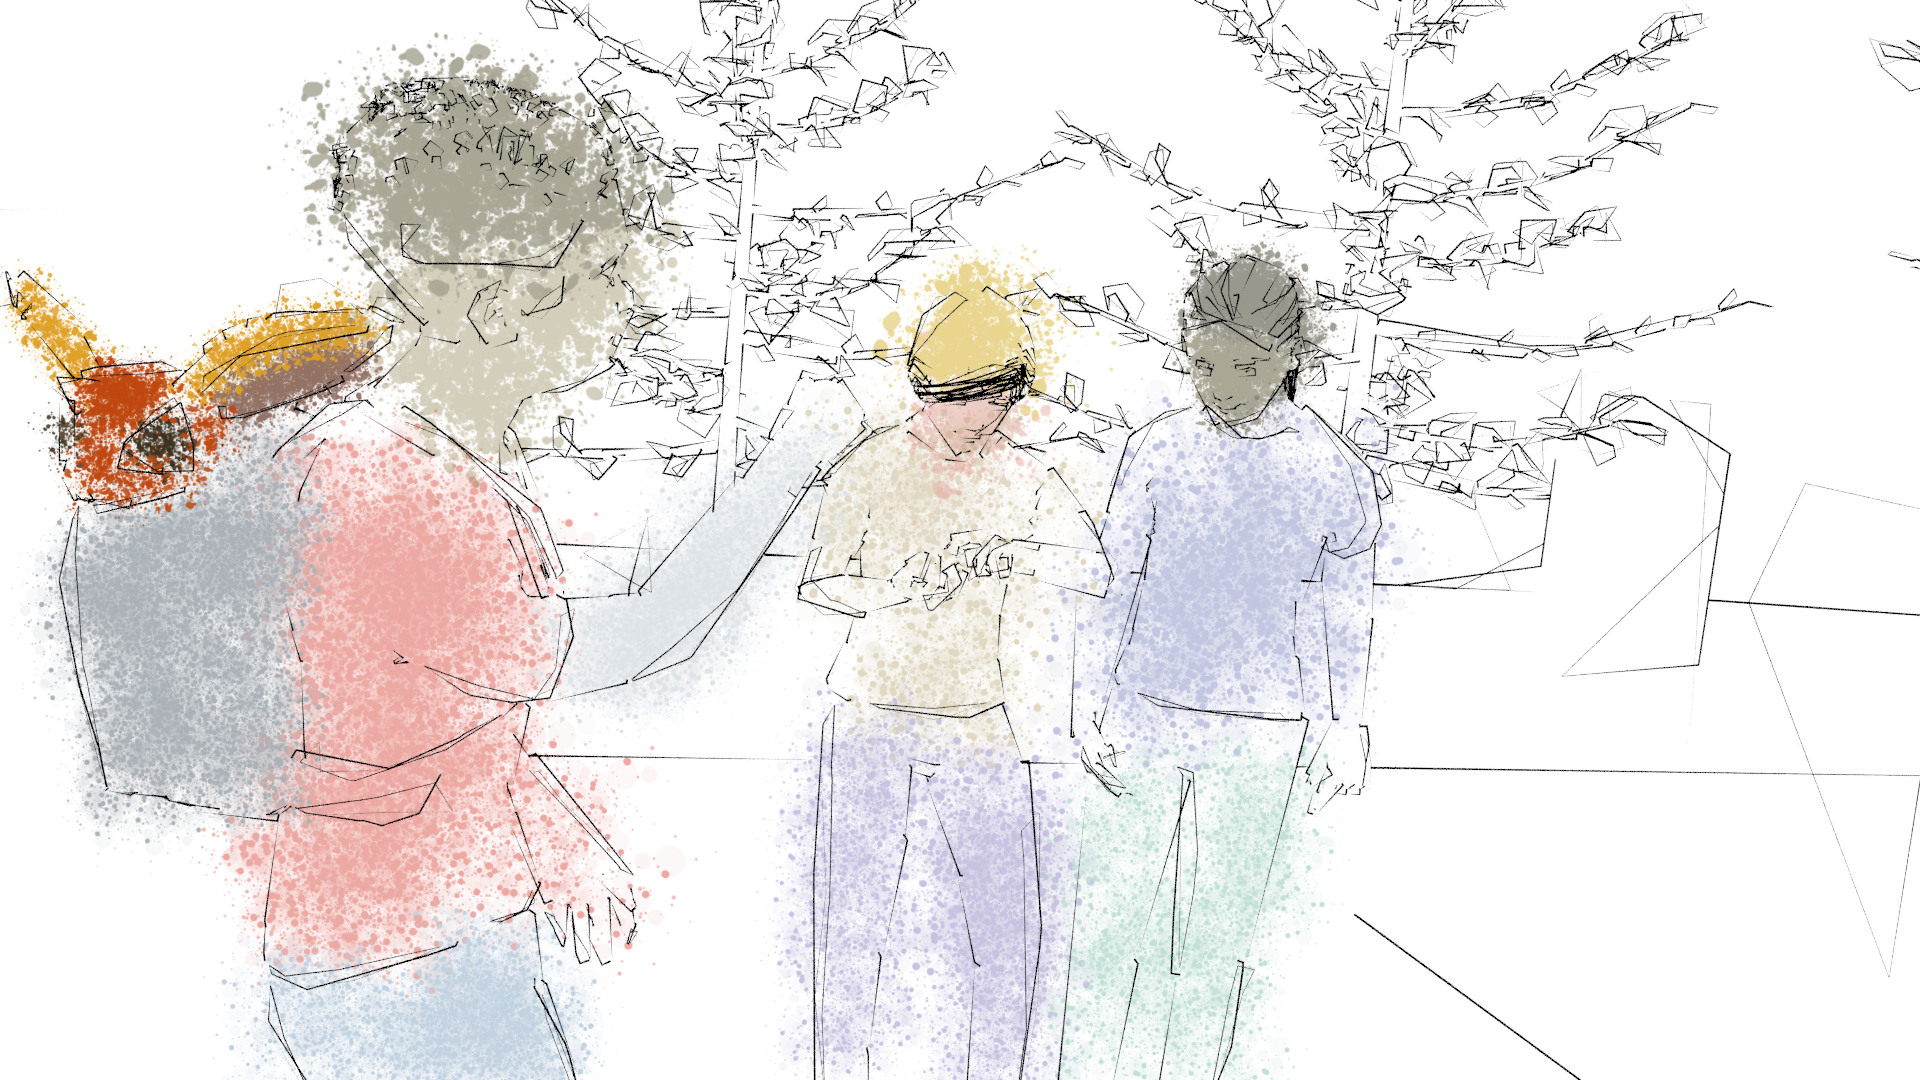
\includegraphics[width=0.9\linewidth]{figs/render5-colors.png}
\end{figure}

\project is a project that aims at helping to build strong human
relationships with the help of technology.

The core idea of the project is to build small companion robots whose
aim is to facilitate human-human interactions. We want to develop these
robots with a particular application in mind: supporting the social and
cultural integration of vulnerable children in a foreign country, and in
particular, migrant children who might lack the otherwise needed support
(shared culture; already well integrated relatives) for a successful
integration.

\subsubsection{Key scientific research questions}

\begin{enumerate}
\item research the role of social influence to scaffold positive human-human
    interactions (including its ethical ramifications) in the context of migrant
    integration;
\item explore how a small robot companion can be endowed with social
    competencies to positively influence human interactions; design and
    implement the corresponding artificial social behaviours;
\item design and build a small rugged and autonomous companion robot that
    realise this goal for child-child interactions; test the technology in
    school with actual migrant children.
\end{enumerate}

\subsubsection{Vision of a novel form of interaction ``human-(robot)-human''}

\paragraph{The case of the social integration of migrant children}

A robot is left with the child when he or she starts their journey in
their new host country, and becomes a companion for the child during the
first months of the integration. Using several mechanisms that are
discussed in this proposal, the robot helps the child to gain
self-confidence, and ultimately engage in successful social interactions
with other children.

Critically, the robot is designed to support the social and cultural
integration of the child \emph{amongst her/his peers}. While the child
might build affective/emotional bonds with the robot over the course of
the support period, the robot behaviour is designed to ensure that these
bonds do not substitute themselves to the interactions with other
children.

The project combines a range of scientific and engineering endeavours to
realise within a 5-years timeframe an ambitious and bold vision for
social robotics in our society. Specifically, the project draws from the
fields of social robotics; human-robot interaction; human-machine
interaction design; and mechatronics.

While the breadth of the proposed project is significant (from
mechatronic design to long-term field testing with vulnerable
populations), the project structure minimizes the cross-dependencies
within the project, avoiding critical failure points that would put the
whole project at risk, and a careful risk assessment is conducted that
includes meaningful mitigation strategies.



%%%%%%%%%%%%%%%%%%%%%%%%%%%%%%%%%%%%%%%%%%%%%%%%%%%%%%%%%%%%%%%%%%%%%%%%%%%
%%%%%%%%%%%%%%%%%%%%%%%%%%%%%%%%%%%%%%%%%%%%%%%%%%%%%%%%%%%%%%%%%%%%%%%%%%%
%%%%%%%%%%%%%%%%%%%%%%%%%%%%%%%%%%%%%%%%%%%%%%%%%%%%%%%%%%%%%%%%%%%%%%%%%%%
\section{Social robots in the society}

\subsection{Psycho-social underpinnings}

Developing a conceptual framework for \emph{robot-supported human-human
interactions} implies a deep understanding of the psycho-social mechanisms at
work in human-human interactions, and in human-robot interactions.

Anthropomorphism is a psychological mechanism by which a human
ascribe human traits to non-human artefacts (here, robots): while the
robot appearance and behaviour can elicit or reinforce these ascription,
it fundamentally originate in the human her/himself~\cite{fink}.


\paragraph{A support for shared understanding}

\emph{Computer Supported Collaborative Learning} (CSCL) researches the cognitive
mechanisms and practical techniques underpinning efficient learning in social
situations. From its very beginning, CSCL research has been following
Roschelle and Teasley's suggestion~\cite{roschelle1995construction} that
collaborative learning has something to do with the process of constructing and
maintaining a \emph{shared understanding} of the task at hand. Building a shared/mutual
understanding refers to the upper class of collaborative learning situations,
those in which students should build upon each other's understanding to refine
their own understanding.  What is expected to produce learning is not the mere
fact that two students build the same understanding but the cognitive effort
they have to engage to build this shared
understanding~\cite{schwartz1995emergence}.

The construction of a shared understanding has been investigated for several
years in psycholinguistics, under the  notion of \emph{grounding}\footnote{Note
that the meaning of \emph{grounding} -- ensuring a shared understanding of a
situation during an interaction -- that we employ in this article must be
distinguished from its meaning in the context of \emph{symbol grounding} as
defined by Harnad~\cite{harnad1990symbol}.}~(Clark,
in~\cite{clark1986referring}).  However, the relevance of grounding mechanisms
for explaining learning outcomes has been questioned in learning sciences. The
monitoring and repair of misunderstanding explains for instance referential
failures in short dialogue episodes but does hardly predict \emph{conceptual
change} (ie the acquisition, acceptation and integration of a new belief into
one's mental model) over longer
sessions~\cite{dillenbourg2006sharing}. The cumulative effect of grounding
episodes can probably be better understood from a socio-cultural perspective:

\begin{quote}
Collaborative learning is associated with the increased
cognitive-interactional effort involved in the transition from \emph{learning to
understand each other} to \emph{learning to understand the meanings of the semiotic
tools that constitute the mediators of interpersonal
interaction}~\cite{baker1999role}
\end{quote}

Along this line, several scholars suggest that CSCL research should go deeper in
the understanding of how partners engage into shared meaning
making~\cite{stahl2007meaning} or \emph{intersubjective} meaning
making~\cite{suthers2006technology}.

Paradoxically, while Clark's theory is somewhat too linguistic from a conceptual
change viewpoint, it is criticized at the same time as being too cognitivist by
some psycholinguists, ie as overestimating the amount of shared knowledge and
mutual representations actually necessary to conduct a dialogue. The fundamental
issue, as old as philosophy, is the degree of coupling between the different
levels of dialogue, mostly between the lexical/syntactical level and the deeper
semantic levels. In~\cite{pickering2006alignment}, Pickering and Garrod argue
that the mutual understanding starts mostly with a \emph{superficial alignment}
at the level of the linguistic representations, due to priming mechanisms, and
that this local alignment may -- in some cases -- lead to a \emph{global
alignment} of the semantic level (\emph{deep grounding}).  For these authors,
the convergence in dialogue, and even the repair of some misunderstandings, is
explained by this mimetic behavior more than by a monitoring of each other's
knowledge: \emph{``...interlocutors do not need to monitor and develop full
common ground as a regular, constant part of routine conversation, as it
would be unnecessary and far too costly. Establishment of full common ground
is, we argue, a specialized and non-automatic process that is used primarily
in times of difficulty (when radical misalignment becomes
apparent).''}~\cite{pickering2006alignment} This view is actually not
incompatible with Clark's \emph{grounding
criterion}~\cite{clark1989contributing}: the degree of shared understanding that
peers need to reach depends upon the task they perform. For instance, a dialogue
between two surgeons might rely on superficial alignment if they talk about
their friends but has to guarantee accurate common grounds when talking about
which intervention will be conducted in which way on which patient.

Deep grounding or shared meaning making requires some cognitive load. For Clark,
what is important is not the individual effort made by the receiver of a
communicative act, but the overall \emph{least collaborative
effort}~\cite{clark1986referring}.  The cost of producing a perfect utterance
may be higher than the cost of repairing the problems that may arise through
misunderstandings. For instance, subjects are less careful about adapting their
utterances to their partner when they know they can provide feedback on his/her
understanding~\cite{schober1993spatial}. Dillenbourg et al. introduced the
notion of \emph{optimal collaborative effort}~\cite{dillenbourg1995evolution} to
stress that misunderstanding should not be viewed as something to be avoided (if
this was possible), but as an opportunity to engage into verbalization,
explanation, negotiation, and so forth.



\paragraph{Developmental pathopsychology}

The false belief experiment that we have mentioned above, was proposed by
Baron-Cohen in the frame of his research on autistic spectrum disorders (he
shows that autistic children seem to actually lack a theory of mind and suggests
this as the primary cause of their social impairments), and Frith and Happé
further note in ~\cite{frith1994autism} that this specific deficit of autism has
led to a large amount of research which proved, in turn, highly beneficial to
the study of the development of theory of mind in general. They reference
in~\cite{frith1994autism} eight such tasks (Table~\ref{mentalizing-tasks}),
identified during the study of social cognition by autistic children. Each of
them is proposed in two versions: one does not require mentalizing, while the
other does require it.  One of these tasks, for example, required children to
distinguish emotions, namely happy/sad faces on one hand (\emph{situation-based}
emotion), and surprised faces on the other (\emph{belief-based}
emotion)~\cite{baron1993children}.  Another task, based on the
\emph{penny-hiding game}, contrasts the two conditions in terms of \emph{object
occlusion} vs.~\emph{information occlusion}~\cite{baron1992out} (we detail it
hereafter). These tasks prototypically illustrate social meta-cognition: one
need to represent and reflect on someone else representations (and not only
perceptions), and they are not addressed by today's research on social robots.

Experimental protocols in research on autistic spectrum disorders are often
striking by their apparent straightforwardness because of the careful choice of
interaction modalities: since autistic children frequently exhibit impairments
beyond social ones (such as motor or linguistic ones), the experiments must be
designed such that they require only basic cognitive skills beyond the social
abilities that are tested. The Sally and Anne task, for instance, requires the
observing child to be able to visually follow the marble, to remember the true
location of the marble, to understand simple questions (``Where will Sally look
for her marble?'' in Baron-Cohen's protocol~\cite{baron1985does}) and eventually
to give an answer, either verbally or with a gesture -- the two first points
being actually explicitly checked through questions: ``Where is the marble
really?'' (reality control question) and ``Where was the marble in the
beginning?'' (memory control question).

Likewise, current social robots have limited cognitive skills (no fast yet fine
motor skills, limited speech production and understanding, limited scene
segmentation and object recognition capabilities, etc.) and such tasks
that effectively test a single cognitive skill (in this case, mentalizing) in
near isolation are of high relevance for experimental social robotics.

\begin{table}[h]
    \centering
    \begin{tabular}{p{0.4\linewidth}p{0.5\linewidth}}
        \toprule
        No mentalizing required           & Mentalizing required          \\
        \midrule
        Ordering behavioural pictures     & Ordering mentalistic pictures~\cite{baron1986mechanical} \\
        Understanding see                 & Understanding know~\cite{perner1989exploration}            \\
        Protoimperative pointing          & Protodeclarative pointing~\cite{baron1989perceptual}     \\
        Sabotage                          & Deception~\cite{sodian1992deception}                     \\
        False photographs                 & False beliefs~\cite{leslie1992domain}                 \\
        Recognizing happiness and sadness & Recognizing surprise~\cite{baron1993children}          \\
        Object occlusion                  & Information occlusion~\cite{baron1992out}         \\
        Literal expression                & Metaphorical expression~\cite{happe1993communicative}       \\
        \bottomrule
    \end{tabular}
    \caption{\small Tasks requiring or not mentalizing to pass, listed by Frith and Happé in~\cite{frith1994autism}}
    \label{mentalizing-tasks}
\end{table}

Frith and Happé's list (Table~\ref{mentalizing-tasks}) is in that regard
especially interesting in that it mirrors pairs of task (ones which do not
require mentalizing with similar ones which do require mentalizing), thus
providing control tasks.  \emph{Object occlusion} vs.~\emph{Information
occlusion} is one example of a (pair of) task(s) which evidence
representation-level perspective taking through \emph{adaptive deception}:
during a simple game, the experimenter adapts its strategy
(deceptive/non-deceptive behaviour) to the representation skills of its child
opponent. The experimental setting is derived from the penny-hiding game
protocol originally proposed by Oswald and Ollendick~\cite{oswald1989role} and
replicated and extended by Baron-Cohen in~\cite{baron1992out}, who describes it
as a two-person game in which the subject is actively involved, either as a
guesser or as a hider. The hider hides the penny in one hand or the other, and
then invites a guess. The game is repeated several time before switching the
roles. Baron-Cohen proposes a specific index to rate the level of the players
based on the idea of \emph{information occlusion}: minimally, the hider must
ensure \emph{object occlusion} (the penny must not become visible to the
guesser), while good hiders, with representation-level perspective taking
skills, develop strategies (like random hand switching or deictic hints at the
wrong hand) to prevent the guesser to find the penny (\emph{information
occlusion}). One could imagine a similar protocol adapted to robotics: the robot
would play the role of the experimenter, adapting on-line its
behaviour to what it understands of the perspective taking capabilities of the
children, and would consequently require \emph{second-order},
\emph{representation-level} perspective taking from the robot.




%%%%%%%%%%%%%%%%%%%%%%%%%%%%%%%%%%%%%%%%%%%%%%%%%%%%%%%%%%%%%%%%%%%%%%%%%%%
%%%%%%%%%%%%%%%%%%%%%%%%%%%%%%%%%%%%%%%%%%%%%%%%%%%%%%%%%%%%%%%%%%%%%%%%%%%
%%%%%%%%%%%%%%%%%%%%%%%%%%%%%%%%%%%%%%%%%%%%%%%%%%%%%%%%%%%%%%%%%%%%%%%%%%%
\section{Companion robots}

One example of a small, rugged robot designed for intensive use in school
environments is Cellulo~\footcite{ozgur2017cellulo}.

\begin{figure}[!htbp]
    \begin{minipage}[b]{.3\linewidth}
        \centering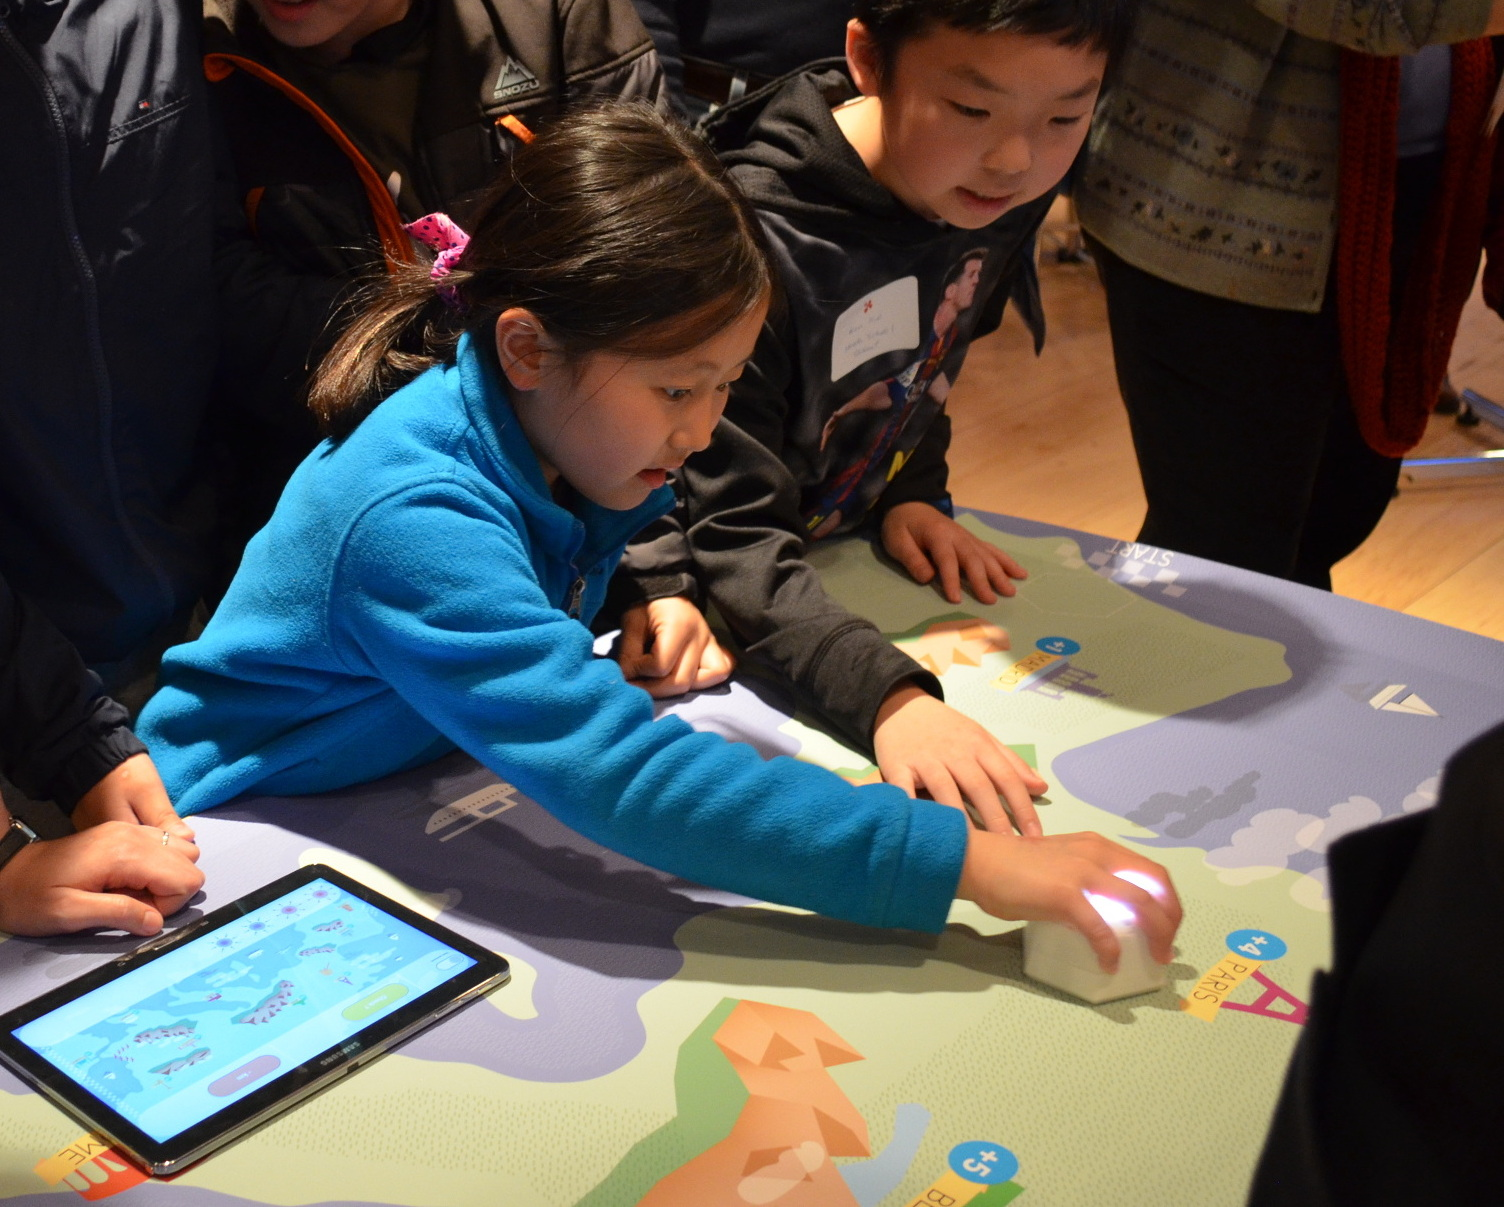
\includegraphics[height=4cm]{figs/cellulo.jpg}
        \subcaption{EPFL's Cellulo robot}\label{fig:cellulo}
    \end{minipage}%
    \hspace{0.5cm}
    \begin{minipage}[b]{.3\linewidth}
        \centering
        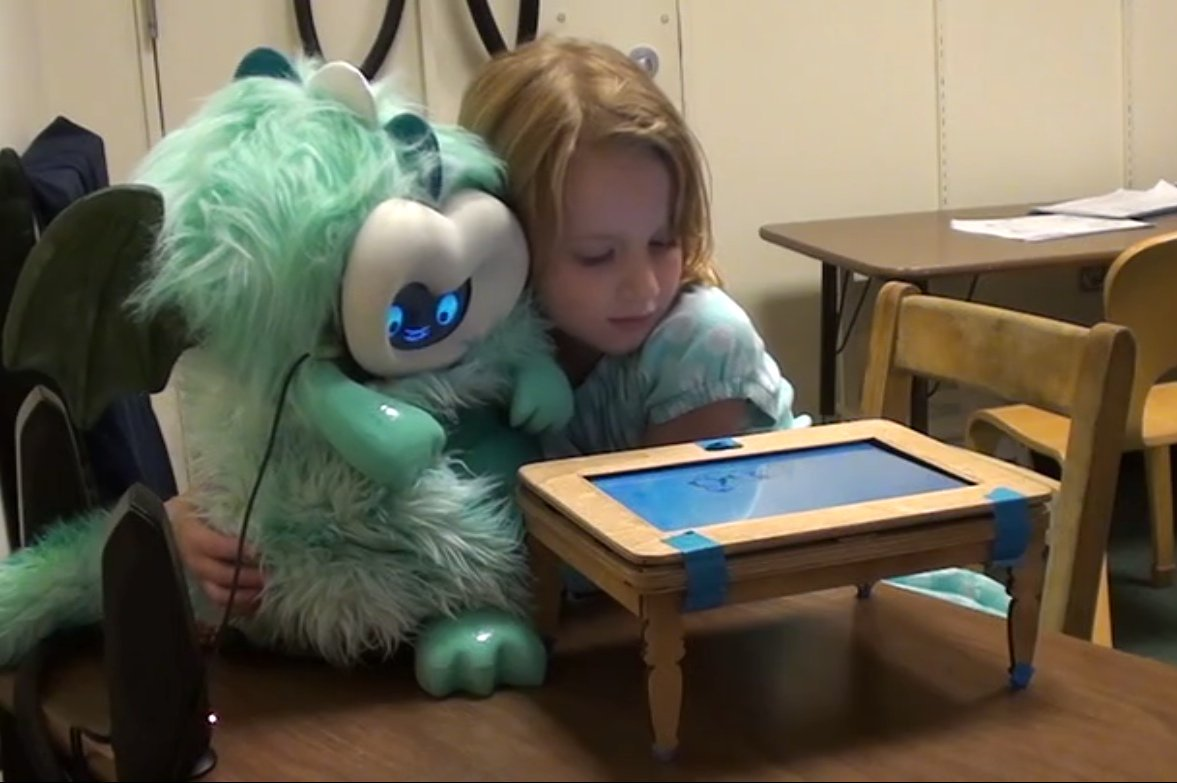
\includegraphics[height=4cm]{figs/tega.jpg}
        \subcaption{MediaLab's Tega robot}\label{fig:tega}
    \end{minipage}
    \hspace{0.5cm}
    \begin{minipage}[b]{.3\linewidth}
        \centering
        %\includegraphics[height=4cm]{figs/ono.png}
        \subcaption{OPSORO's Ono robot}\label{fig:ono}
    \end{minipage}
    \caption{Existing research-level companion robots}\label{fig:research-robots}
\end{figure}

\begin{figure}[!htbp]
    \begin{minipage}[b]{.3\linewidth}
        \centering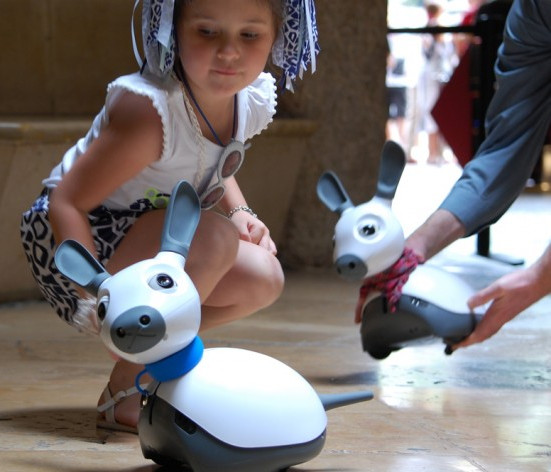
\includegraphics[height=4cm]{figs/miro.jpg}
        \subcaption{Consequential's Miro robot}\label{fig:miro}
    \end{minipage}%
    \hspace{0.1cm}
    \begin{minipage}[b]{.3\linewidth}
        \centering
        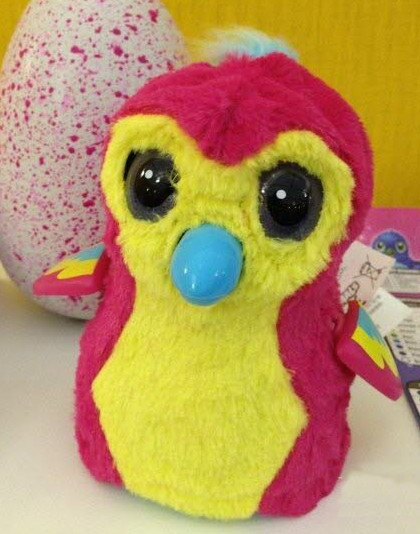
\includegraphics[height=4cm]{figs/hatchnimals.jpg}
        \subcaption{SpinMaster's Hatchimals}\label{fig:hatchimals}
    \end{minipage}%
    \hspace{0.1cm}
    \begin{minipage}[b]{.3\linewidth}
        \centering
        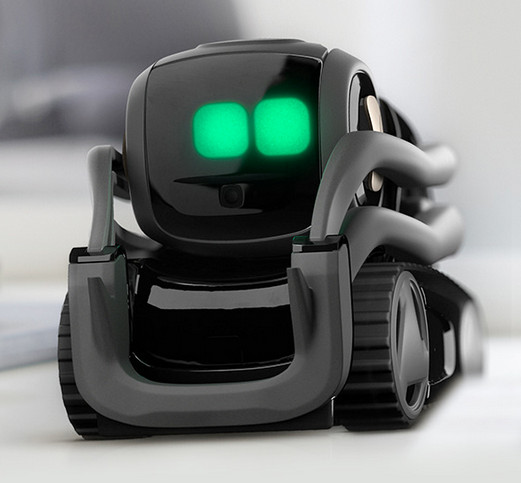
\includegraphics[height=4cm]{figs/anki-vector.jpg}
        \subcaption{Anki's Vector}\label{fig:vector}
    \end{minipage}
    \caption{Existing commercial companion robots}\label{fig:commercial-robots}
\end{figure}



\begin{figure}
    \centering
    
\includegraphics[width=0.9\linewidth]{figs/wizme+dolls}
    \caption{Early prototyping for the \project: a pet-like robot that could
    mediate child-child interactions}
    \label{}
\end{figure}


%%%%%%%%%%%%%%%%%%%%%%%%%%%%%%%%%%%%%%%%%%%%%%%%%%%%%%%%%%%%%%%%%%%%%%%%%%%
\section{Social situation assessment}

\begin{figure}
\centering
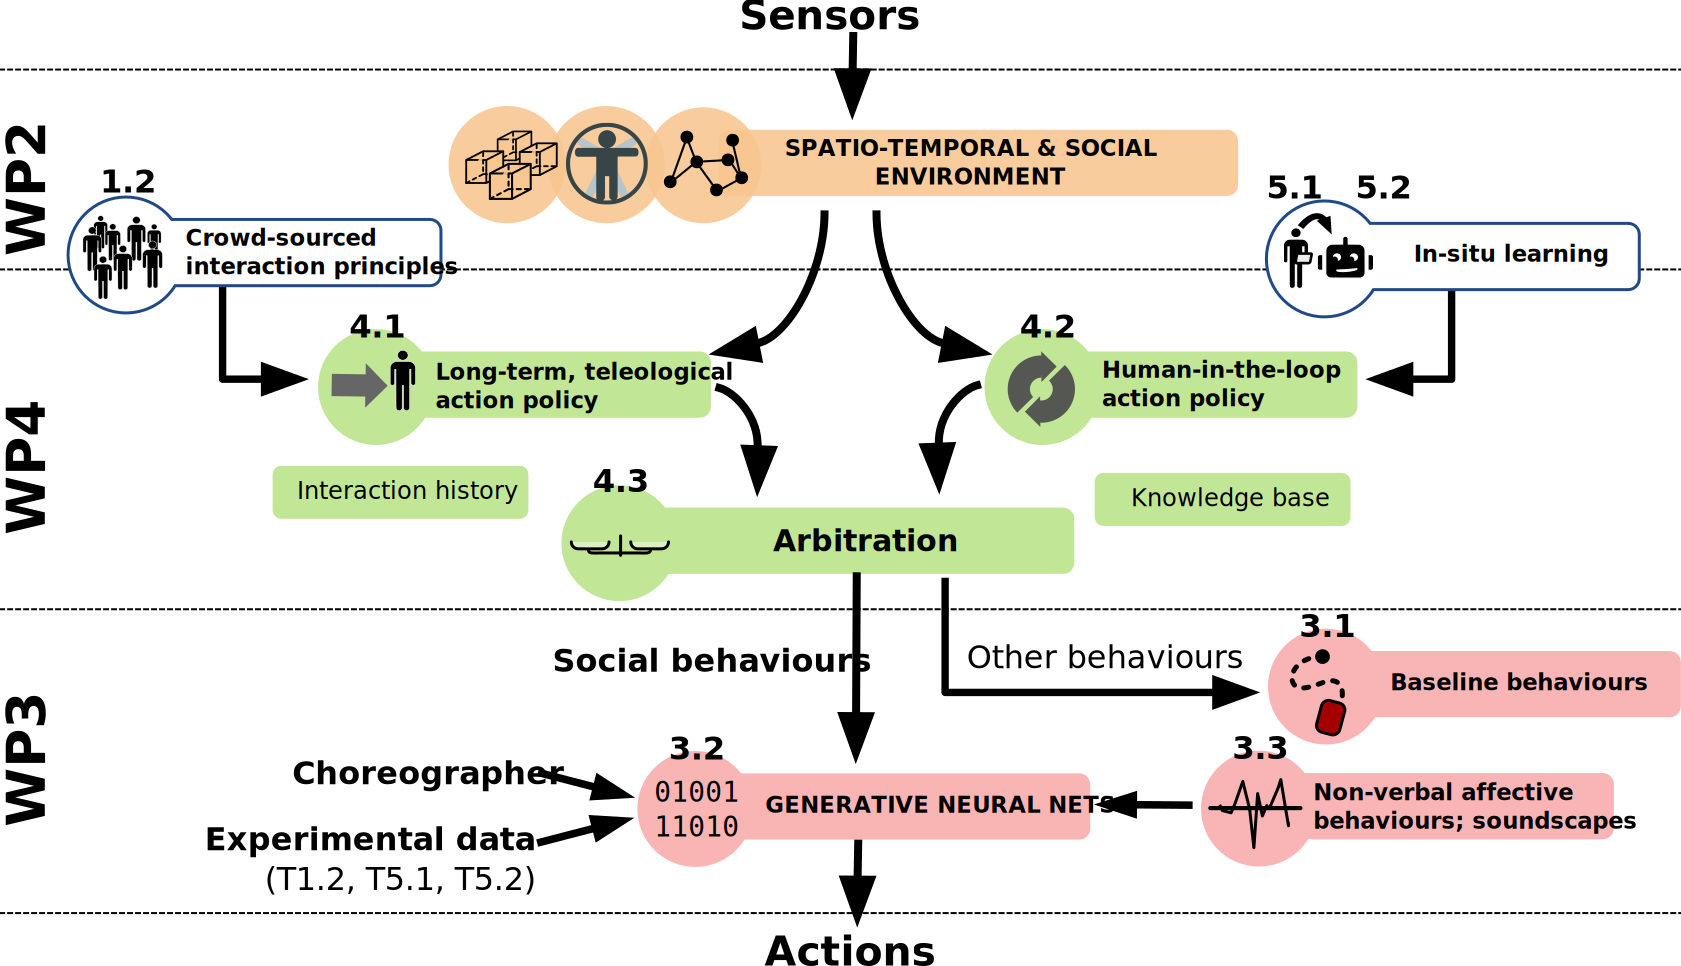
\includegraphics[width=0.9\linewidth]{figs/archi}
\caption{Overview of the technical architecture enabling social situation
    assessment: social situation assessment builds on strong \emph{situation
    assessment}, on top of which humans and human interactions are layered.}
\label{fig:social-situation-assessment}
\end{figure}


%%%%%%%%%%%%%%%%%%%%%%%%%%%%%%%%%%%%%%%%%%%%%%%%%%%%%%%%%%%%%%%%%%%%%%%%%%%
\section{Social influence}

\begin{figure}[!htbp]
\centering
    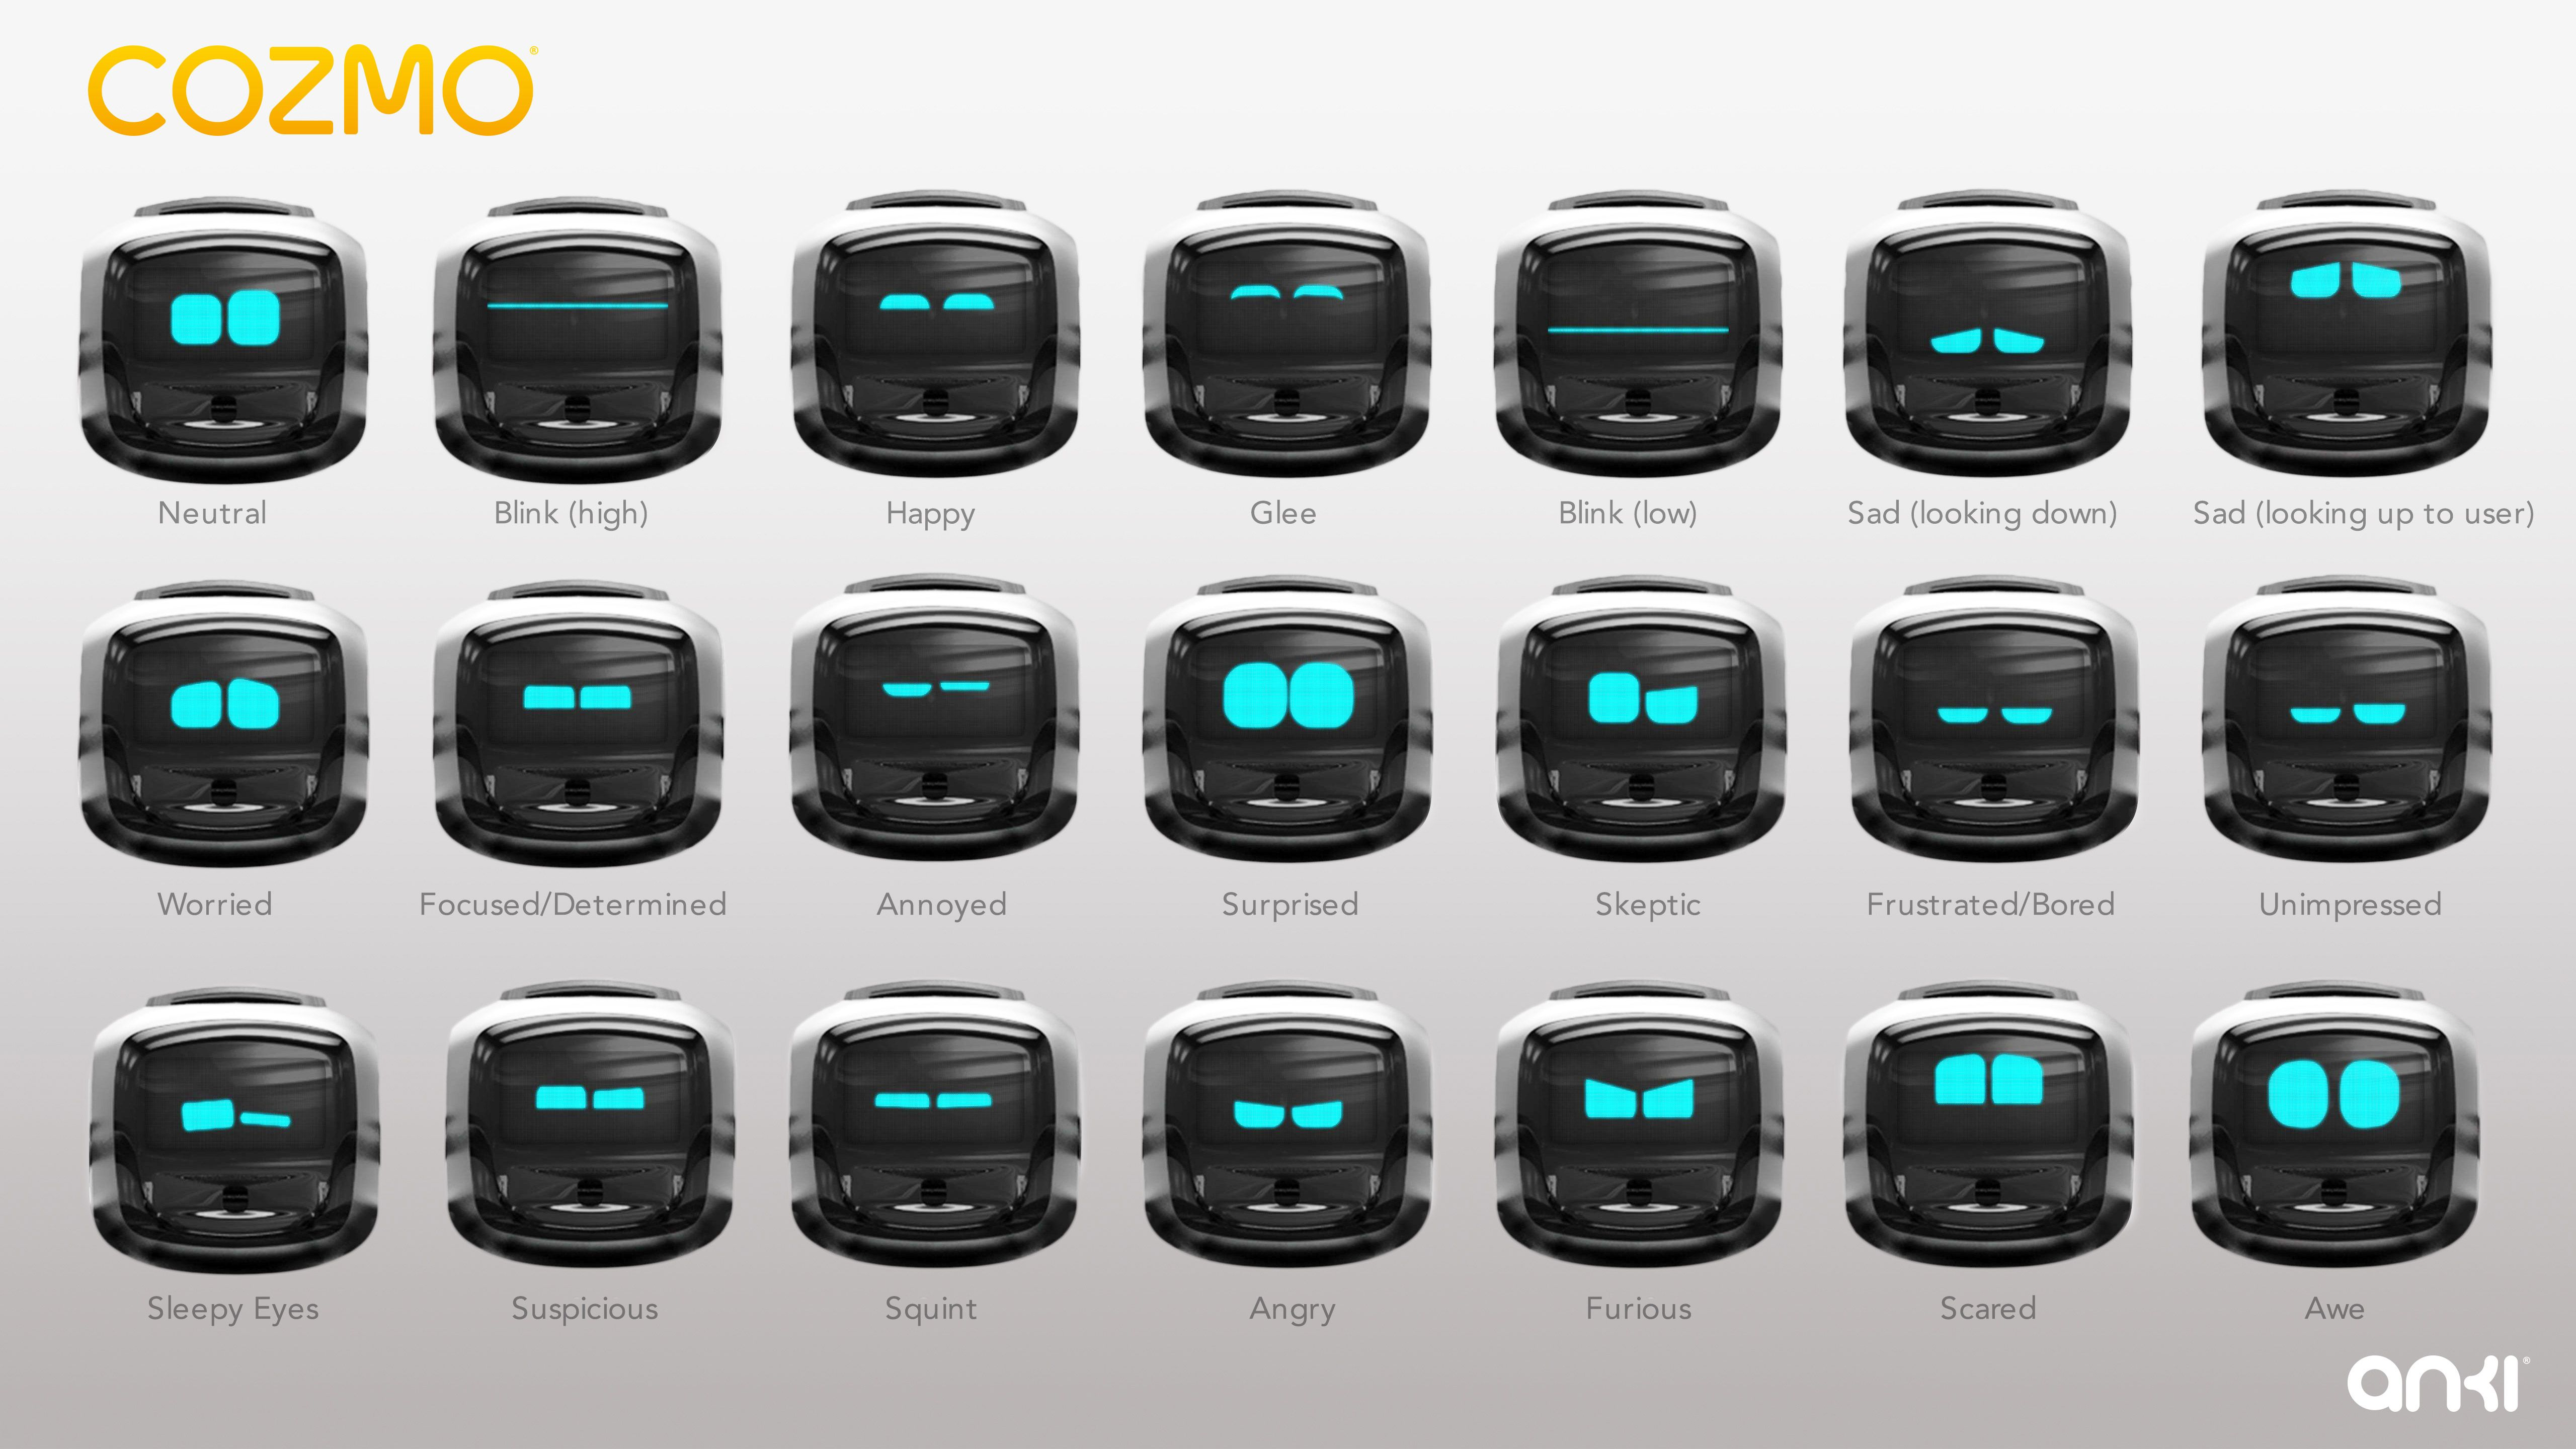
\includegraphics[width=0.7\textwidth]{figs/cozmo-expression-sheet.jpg}
\caption{Cozmo facial expressions}
\end{figure}


\section{Impact}\label{impact}

\subsection{Impact on society and technology: building an inclusive society}


\project will deliver new and fundamental knowledge to the fields of robotics,
computer science and psychology, in addition to improving trans-disciplinary
understanding between these disciplines. More specifically, the project will
contribute to a better understanding of the following research areas:
human-robot interaction; human-machine interaction; human error making and
handling in assembly tasks; theory of mind and its transfer to cognitive robots;
natural language processing; explainability and language generation; machine
vision and human activity detection; and action planning under uncertainty. New
interaction paradigms will be developed for handling error situations where
machines interact with non-expert humans. The integration of perception and
sensing into cognitive robot architectures will be critically reviewed and
extended. Novel, empirically informed methods to transfer findings from
human-human interaction studies to human-machine interactions will be developed.
Furthermore, the national and international psychology, robotics and computer
science research communities will benefit from the project results. We will
publish \project results in interdisciplinary and discipline-specific journals
and conferences, and organise \project-themed workshops. Please refer to Section
\ref{sec:impact} about our concrete action plan to maximise impact. 




Academically, the \project project represents a timely combination of
very recent advances in supervised machine learning for social robot
behaviour with a creative and interdisciplinary approach to the design
and automation of social robot behaviour. We therefore expect to publish
results in high-class scientific journals and conferences.

The dataset of social behaviours and social signals we will create and
distribute represents a one-in-a-kind resource for the human robot
interaction community, and the human data collection will be
transferable to research in other domains such as human-computer
interaction.

As \project will be deployed in a living lab environment, there is
significant scope for public outreach/engagement and media coverage,
which we will work with the BRL's media manager to maximise.

%%%%%%%%%%%%%%%%%%%%%%%%%%%%%%%%%%%%%%%%%%%%%%%%%%%%%%%%%%%%%%%%%%%%%%%%%%%
%%%%%%%%%%%%%%%%%%%%%%%%%%%%%%%%%%%%%%%%%%%%%%%%%%%%%%%%%%%%%%%%%%%%%%%%%%%
%%%%%%%%%%%%%%%%%%%%%%%%%%%%%%%%%%%%%%%%%%%%%%%%%%%%%%%%%%%%%%%%%%%%%%%%%%%
\chapter{B2.b Methodology}\label{research-methodology}

\eu{Describe the proposed methodology in detail including any key intermediate
goals. Explain and justify the methodology in relation to the state of the art,
and particularly novel or unconventional aspects addressing the
'high-risk/high-gain' balance. Highlight any intermediate stages where results
may require adjustments to the project planning. In case you ask that team
members are engaged by another host institution their participation has to be
fully justified by the scientific added value they bring to the project.}

%%%%%%%%%%%%%%%%%%%%%%%%%%%%%%%%%%%%%%%%%%%%%%%%%%%%%%%%%%%%%%%%%%%%%%%%%%%
\section{Data-driven continuous behaviour generation}


At a time where companion robots are coming to the market, one important
question remains fully open: how to design robot behaviours that foster
lasting engagement? A vast body of academic literature identifies that
robots evoke an initial phase of high user engagement (the
\emph{novelty} phase) that vanishes as the user realises that the robot
is actually quite predictable and repetitive. The \emph{agency}
initially ascribed by the user to the robot quickly fades (Lemaignan et
al. 2014), leading to critical user disengagement from the technology.

%\begin{wrapfigure}[23]{l}{6.5cm}
\begin{figure}
    \centering
    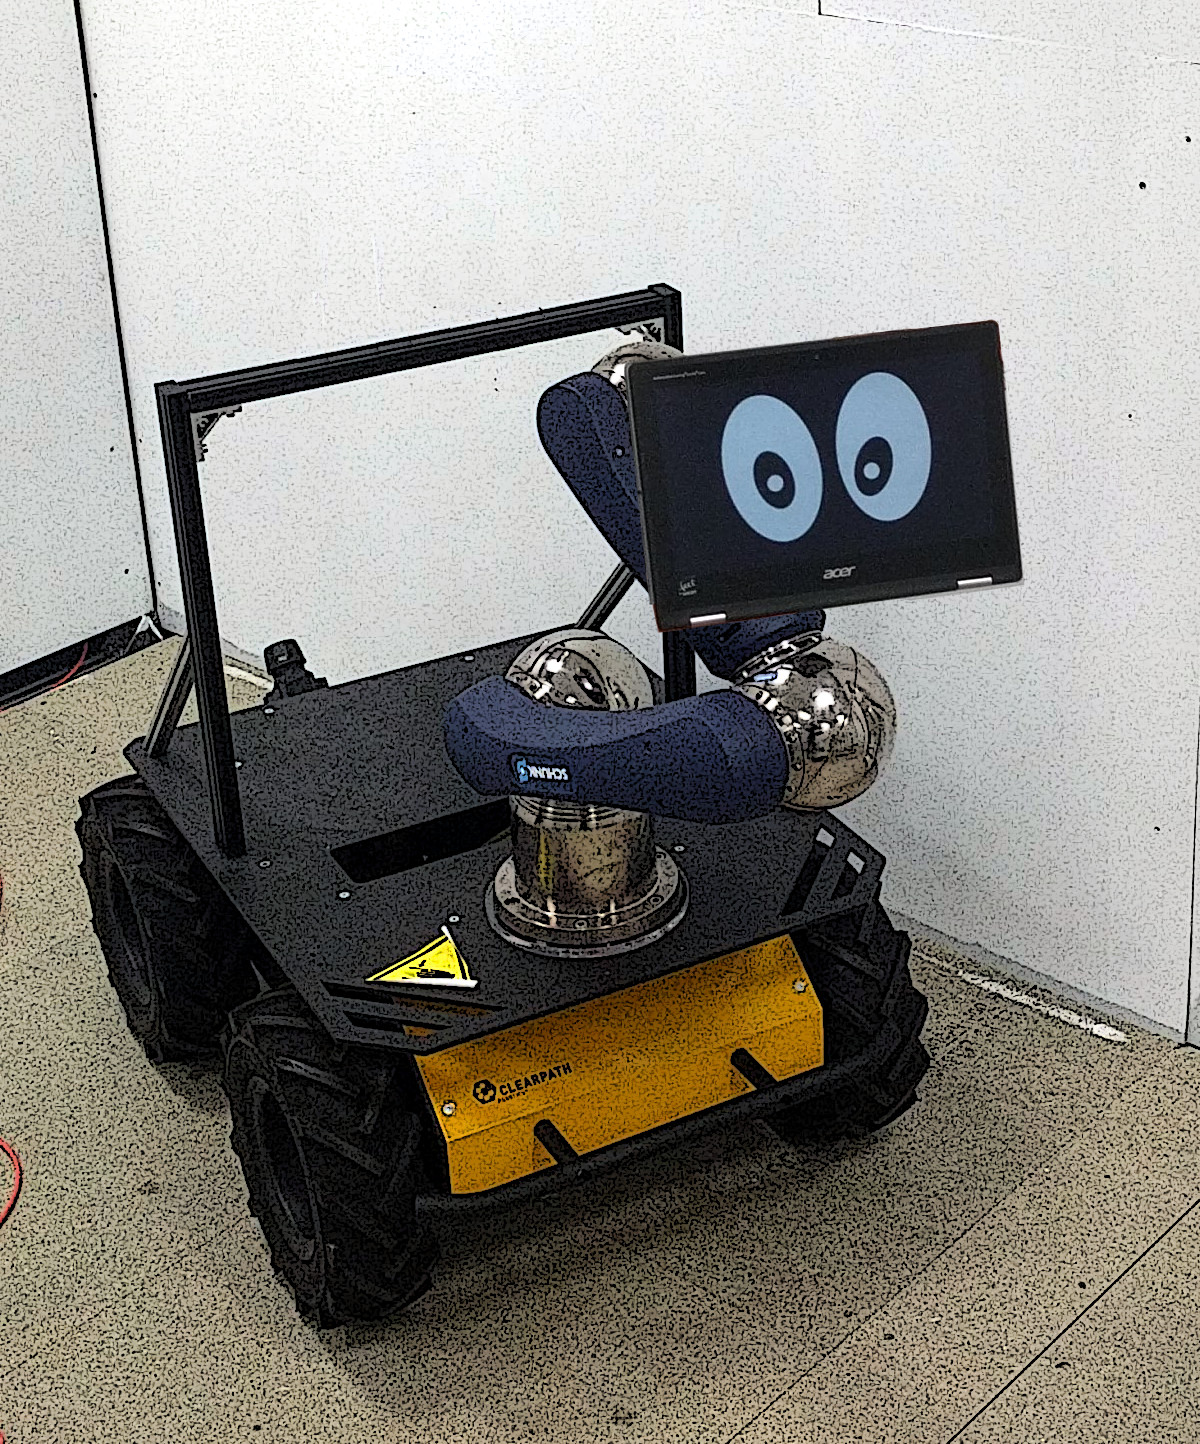
\includegraphics[width=0.5\paperwidth]{figs/husky.jpg}
    \caption{\label{fig:robot}
    Provisional appearance of the \project robot that we ill use to collect
    data. A tablet, displaying facial animations, is mounted on a robotic arm.
    It can freely orient its `gaze' and use expressive movements. The mobile
    base (a Segway Husky) can autonomously navigate in the various parts of the
    BRL open-space}
\end{figure}
%\end{wrapfigure}

The (often limited) library of behaviours available to the robot is
often cited as a key factor in causing this issue. However, another,
more profound issue affecting long term engagement with robot companions
is the question of \emph{purpose.} Without clear \emph{purpose}, social
robot companions can lack \emph{usefulness}. Indeed, robot
\emph{companions} might not have explicit goals that would dictate or
motivate their behaviours: they aim at providing a social presence, a
social comfort, as cats or dogs would do, without necessarily being
goal-oriented.

Recent attempts -- and failures -- to convert social robotics research
into commercial platforms (Jibo, Kuri and most recently Anki's Cozmo and
Vector robots) reflect exactly this, with reasons for their failure
typically citing an under-delivery of the user experience they promised,
and/or the lack of a `real need' to justify their price point. The
\project project addresses these two key issues by:

\begin{enumerate}
\def\labelenumi{\arabic{enumi}.}
\item
  Taking inspiration from human-pet relationships which also have no
  explicit \emph{purpose} beyond their potential for enjoyable,
  \emph{affective} interactions;
\item
  Working with creative professionals who excel at storytelling and
  emotional engagement to overcome the problems in sustaining
  engagement, as proposed by Hoffman\footnote{\url{https://spectrum.ieee.org/automaton/robotics/home-robots/anki-jibo-and-kuri-what-we-can-learn-from-social-robotics-failures}};
\item
  Blending these two sources of inspiration using a radically novel
  combination of immersive teleoperation and machine learning.
\end{enumerate}

The project is \emph{not} about replicating a pet's behaviour per se. It
is instead about identifying, modeling and automatically generating the
social behaviours required to recreate pet-like social dynamics between
robots and humans, drawing inspiration from ethology (Stanton, Sullivan,
and Fazio 2015). Using animal behaviours to inform the design of robots
is not new, the most remarkable example being the Sony AIBO robot dog,
whose behaviours were directly designed around those of actual dogs
(Arkin et al. 2003). However, to go beyond the repetitive interactions
associated with such robots, we propose to employ a creative
professional to actively participate in design and automation of \project
behaviour. The concept of using creative professionals to `teach' social
robot behaviour is not new either (Knight and Gray 2012), however it is
only recent advances in human-in-the-loop, online machine learning that
make this type of real-time `social training' a feasible approach to
generating and automating engaging social behaviours (Senft et al.
2019).

Our project has the following goals, addressed by the workplan presented
below:

\begin{enumerate}
\def\labelenumi{\arabic{enumi}.}
\item
  assemble a non-anthropomorphic social robot that can autonomously
  navigate in a complex and living lab environment, taking inspiration
  from ethology to inspire the robot's behaviour;
\item
  develop an immersive teleoperation system, enabling a creative
  professional to `take control' of the robot (i.e.~puppet the robot) in
  a completely intuitive way (using whole body motion tracking);
\item
  record (and make publicly available) a large dataset of social
  behaviours (created through immersive teleoperation) that foster
  long-term social and affective engagement. The dataset will also
  include the social \emph{signals} implicitly used by the puppeteer to
  drive his/her choice of actions (recorded through eg eye-tracking);
\item
  using machine learning, map these social signals (input state) to the
  robot behaviours (output state) such that the robot can operate
  autonomously.
\end{enumerate}

A creative professional (puppeteer, dancer or comedian --
corresponding financial compensation is budgeted) will join the group.
First she/he will take part to a one-week co-design workshop (4) aiming
at finalising the immersive teleoperation controller and the behaviours
of the robot. Then, she/he will interact for about 4 hours a day during
a month, with the BRL lab members (200+ researchers). She/he will do so
by remotely operating the robot (5) from an (out-of-sight) control room
(the BRL CAVE room). The aim will be for the puppeteer to pro-actively
engage with people in the lab, attempting to engage in \emph{social,
affective} interactions. This will be achieved by creating/inventing
in-situ a new `grammar' of social behaviour, loosely inspired by those
of cats and other pets. These interactions will be fully recorded
(including eye-tracking on the puppeeter) (6), in order to create a
unique dataset of complex social interactions, suitable for machine
learning. The PI has already extensive experience in recording such
datasets (see (Lemaignan et al. 2018) for instance).

%\begin{wrapfigure}[17]{l}{8cm}
\begin{figure}
    \centering
    
\includegraphics[width=0.8\paperwidth]{figs/dev.pdf}
    \caption{\label{fig:support}
    Social behaviours will be learned from immersive `puppetering' of the
    robot, performed by a professional actor. The `puppetering' takes place
    in a CAVE (or VR) environment, where what the robot `sees' and `hears'
    is streamed live}
\end{figure}
%\end{wrapfigure}

Over the following four months, a deep neural network will be designed
and trained (7) for the regression task of generating continuous social
behaviours from perceived social signals. In parallel, a software
controller will be developed (8) to enable generic autonomous
capabilities (like autonomous navigation) for which the BRL has
extensive expertise.

Finally, the last four months will be dedicated to in-situ testing of
the autonomous system (9). We will seek to conduct a large scale study
within the lab, over a period of several weeks. For this study, the
robot is expected to be fully autonomous. However sufficient amount of
time is planned for additional iterations on the development of the
robot controller if deemed necessary. We aim at publishing the results
of this main study shortly after the end of the one-year period.


%%%%%%%%%%%%%%%%%%%%%%%%%%%%%%%%%%%%%%%%%%%%%%%%%%%%%%%%%%%%%%%%%%%%%%%%%%%
\subsection{Evidence-based research: demonstrable usefulness of social robots in
real-world, complex scenarios}


Critically, the scientific investigation of these questions (\emph{conceptual
framing of robot-supported human-human interaction}, \emph{socially-driven
cognitive architecture},  \emph{online social situation assessment and social
behaviour generation}) has to be
grounded in real-world applications. Indeed, two complex, high impact
applications are detailed in the project. The first one takes place in
Bristol's Children Hospital: a social robot will be permanently deployed in one
of ward, supporting isolated children who suffer long-term conditions, in close
cooperation with the hospital staff. The second one involves the deployment of 
social robots in special need schools (SEN schools) in Bristol. Building on a
rigorous participatory approach involving the school teachers, as well as the
parents, we will seek to integrate the robot in the daily life of the school,
supporting the development of the students' physical and social skills.

These two applications, detailed hereafter, aim at supporting
socially-vulnerable populations: this entails specific risks (detailed and
addressed in the Section~\ref{risks}), but also offers a unique opportunity to
demonstrate in a real-world, impactful case, how social robots can effectively
have a positive, ethical impact, and support in-fine stronger, richer
human-human interactions.



\TODO{probably useful to give specific examples of interventions}

\subsection{Application 1: A robot companion at the children's hospital}

\subsection{Application 2: Social robots in SEN schools}

\TODO{explain that these 2 large experiments will be scaffolded by many smaller
ones}

\subsection{Experimental deployments: risks and mitigations}

These two application scenarios are ambitious and inherently risky, as they
target vulnerable populations. However, first, demonstrating the
importance of advanced social modelling, and convincingly proving the
effectiveness of our approach does require accordingly complex social
situations, and complex social dynamics. The two scenarios, which complement
each other, provide both.

Second, working with vulnerable populations, in constrained and complex
environments (children hospital and SEN schools) adds significant risks to the
project. But it is also what make the project in the unique position of
delivering a high societal impact: a direct positive impact on children's
lives (we anticipate 100+ hospitalised children and 50+ refugee children
interacting over long periods of time with a robot over the course of the
project), and a broader impact on the society, showing how robots can have a
lasting, strong, positive impact on the society, also establishing the idea of
\emph{robots supporting human interactions} instead of dehumanising our social
relationships.

The two main mitigations are (1) early and continuous engagement with the
stakeholders, and (2) the decoupling of the two applications, meaning that the
risks associated to each of them do not impact the other one.

Early engagement will be ensured by relying on a participatory design
methodology, involving all the stakeholders from the onset of the project; the
methodology will involve regular joint workshops; on-site (hospital and refugee
camps) research stay including engagement with the staff/charities and the
children themselves; use of art-based participatory techniques like puppetering.
I will also perform field testing early on in the project, relying if necessary
on provisional robot platforms available at the host institution (for instance,
Softbank Nao and Pepper). This user-centered approach will be championed by one
of the post-doc recruited on the project, who will have recognised expertise in
user-centered design.


The Principal Investigator, Dr.  Séverin Lemaignan, has been working for 12+
years in human-robot interaction, and over the last 6 years, specifically in the
field of child-robot interaction.  His profile is both highly technical, with
hundreds of hardware and software contributions to the worldwide robotic
community; and highly experimental, running dozens of studies and experiments
with children, including long-term ones, in muliple schools and in healthcare
environments. He is in a unique position to deliver both a scientific
breakthrough on social situation assessment for robots, and a high-impact
societal change.

%%%%%%%%%%%%%%%%%%%%%%%%%%%%%%%%%%%%%%%%%%%%%%%%%%%%%%%%%%%%%%%%%%%%%%%%%%%
%%%%%%%%%%%%%%%%%%%%%%%%%%%%%%%%%%%%%%%%%%%%%%%%%%%%%%%%%%%%%%%%%%%%%%%%%%%
\section{Interdisciplinarity}



%%%%%%%%%%%%%%%%%%%%%%%%%%%%%%%%%%%%%%%%%%%%%%%%%%%%%%%%%%%%%%%%%%%%%%%%%%%%%%%%%%%%%%%%
%%%%%%%%%%%%%%%%%%%%%%%%%%%%%%%%%%%%%%%%%%%%%%%%%%%%%%%%%%%%%%%%%%%%%%%%%%%%%%%%%%%%%%%%
%%%%%%%%%%%%%%%%%%%%%%%%%%%%%%%%%%%%%%%%%%%%%%%%%%%%%%%%%%%%%%%%%%%%%%%%%%%%%%%%%%%%%%%%
\newpage
\section{Workplan and intermediate targets}\label{workplan}


%%%%%%%%%%%%%%%%%%%%%%%%%%%%%%%%%%%%%%%%%%%%%%%%%%%%%%%%%%%%%%%%%%%%%%%%%%%%%%%%%%%%%%%



\subsubsection{Project structure}

\begin{table}[!htbp]
    \begin{tabular}{@{}p{1cm}p{6cm}p{2cm}p{2cm}p{1.5cm}p{1.5cm}p{1.5cm}@{}}
\toprule
\textbf{WP} & \textbf{Work package title} & \textbf{Lead participant No} & \textbf{Lead participant short name} & \textbf{Person-Months} & \textbf{Start month} & \textbf{End month} \\ \midrule
1                        & \wpOne                      &                              &                                      &                        &                      &                    \\
2                        & \wpTwo                      &                              &                                      &                        &                      &                    \\
3                        & \wpThree                    &                              &                                      &                        &                      &                    \\
4                        & \wpFour                     &                              &                                      &                        &                      &                    \\
5                        & \wpFive                     &                              &                                      &                        &                      &                    \\
6                        & \wpSix                      &                              &                                      &                        &                      &                    \\
7                        & \wpSeven                      &                              &                                      &                        &                      &                    \\
                         &                             &                              &                                      & \textbf{Total months}  &                      &                    \\ \bottomrule
\end{tabular}
\end{table}


\subsection{Work package 1: \wpOne}

%\begin{table}[!htbp]
%\centering
%\begin{tabular}{|l|p{1.5cm}|p{1.5cm}|p{1.5cm}|p{1.5cm}|p{1.5cm}|p{1.5cm}|p{1.5cm}|}
%\hline
%Work package number            & 1 & \multicolumn{3}{l|}{Lead beneficiary} & \multicolumn{3}{l|}{\bf BRL} \\ \hline
%Work package title             & \multicolumn{7}{l|}{\wpOne}                                             \\ \hline
%Participant number             &     &         &         &                  &       &       &      \\ \hline
%Short name of participant      &     &         &         &                  &       &       &      \\ \hline
%Person/months per participant: &     &         &         &                  &       &       &      \\ \hline
%Start month                    & \multicolumn{3}{l|}{}  & End month        & \multicolumn{3}{l|}{} \\ \hline
%\end{tabular}
%\end{table}


\textbf{Objectives:}

\textbf{Description of work:}

\ldots{}description\ldots{}

\task{1.1}{}

\vspace{0.5cm}\textbf{Deliverables:}

\begin{itemize}

\item   \emph{Deliverable D1.1} (Month 2): website and logo
\end{itemize}

\subsection{Work package 2: \wpTwo}

\textbf{Objectives:}
\textbf{Description of work:}

\ldots{}description\ldots{}

\task{2.1}{Identification of the dimensions of social influence for human interpersonal interactions}

\task{2.2}{Ethics of social influence}
Blah blah

\task{2.3}{Study 1 -- Socially influencing companion robot}
First study, using Anki's Vector robot.

\vspace{0.5cm}\textbf{Deliverables:}

\begin{itemize}
    \item \D{2.1}{12}{great report}
\end{itemize}

\subsection{Work package 3: \wpThree}

\textbf{Objectives:}

\begin{itemize}
    \item refine interaction modalities (in
    particular, the non-verbal speech), details cross-modal interactions,
    define interaction patterns with the child
\end{itemize}

\ldots{}description\ldots{}

\task{3.1}{Analysis of needs}
\task{3.2}{Cross-cultural interactions}

\vspace{0.5cm}\textbf{Deliverables:}

\begin{itemize}
    \item \D{3.1}{12}{great report}
\end{itemize}

\subsection{Work package 4: \wpFour}


\begin{itemize}
    \item long term interaction
    \item one full day of autonomy
    \item rugged \footcite{ozgur2017cellulo, hostettler2016realtime}
    \item child friendly: mechanical constraints~\footcite{ozgur2016permanent} + design
\end{itemize}


\textbf{Description of work:}

Develop a novel platform, including:

\begin{itemize}
    \item chassis
    \item power autonomy for one day
    \item on-board compute suitable for deep learning (NVidia Xavier?)
    \item vision (embedded RGB-D camera)
    \item audio processing
\end{itemize}

\ldots{}

\task{4.1}{Physical design of the robot companion}
\task{4.2}{Interaction design}
\task{4.3}{Mechatronics \& Sensing}
\task{4.4}{On-board data processing}
\task{4.5}{System integration}

\begin{itemize}
    \item \D{4.1}{12}{great report}
\end{itemize}

\subsection{Work package 5: \wpFive}


\textbf{Objectives:}

\textbf{Description of work:}

\ldots{}description\ldots{}

\task{5.1}{Multi-modal communication}
\task{5.2}{Social awareness}
\task{5.3}{Machine learning of social behaviours}
\task{5.4}{Social controller}

\vspace{0.5cm}\textbf{Deliverables:}

\begin{itemize}
    \item \D{5.1}{12}{great report}
\end{itemize}

\subsection{Work package 6: \wpSix}


\textbf{Objectives:}

\textbf{Description of work:}

\ldots{}description\ldots{}

\task{6.1}{Academic dissemination}
\task{6.2}{General public dissemination}
\task{6.3}{Commercial exploitation}

\vspace{0.5cm}\textbf{Deliverables:}

\begin{itemize}
    \item \D{6.1}{12}{website and logo}
\end{itemize}

\subsection{Work package 7: \wpSeven}

\textbf{Objectives:}

\textbf{Description of work:}

\ldots{}description\ldots{}

\task{7.1}{Academic dissemination}
\task{7.2}{General public dissemination}
\task{7.3}{Commercial exploitation}

\vspace{0.5cm}\textbf{Deliverables:}

\begin{itemize}
    \item \D{7.1}{12}{website and logo}
\end{itemize}


\subsection{Deliverables overview}\label{deliverables-overview}

\begin{table}[!htbp]
\caption{List of deliverables}
\begin{tabular}{@{}lllllll@{}}
\toprule
\textbf{Deliverable} & \textbf{Deliverable name} & \textbf{Work package No} & \textbf{Lead participant short name} & \textbf{Type} & \textbf{Dissemination level} & \textbf{Delivery date} \\ \midrule
D1.1                 &                           &                          &                                      &               &                              &                        \\
D1.2                 &                           &                          &                                      &               &                              &                        \\
D2.1                 &                           &                          &                                      &               &                              &                        \\
...                  &                           &                          &                                      &               &                              &                        \\ \bottomrule
\end{tabular}
\end{table}

Type:

\begin{itemize}

\item   R: Document, report (excluding the periodic and final reports)
\item   DEM: Demonstrator, pilot, prototype, plan designs
\item   DEC: Websites, patents filing, press \& media actions, videos, etc.
\item   OTHER: Software, technical diagram, etc.
\end{itemize}

Dissemination level:

\begin{itemize}

\item   PU = Public, fully open, e.g.~web
\item   CO = Confidential, restricted under conditions set out in Model Grant
  Agreement
\item   CI = Classified, information as referred to in Commission Decision
  2001/844/EC.
\end{itemize}

\subsection{Gantt chart}\label{gantt-chart}

\begin{landscape}
%%%%%%%%%%%%%%%%%
%%
%% Task dependencies
%%
%% Task...        depends on Task...
%% T1.3           T1.1
%% T1.3           T1.2
%% T1.2           T2.2 (user interface)
%% T3.3           T2.3
%%

\definecolor{barcolor}{RGB}{153,204,254}
\definecolor{linkred}{RGB}{165,0,33}
%\renewcommand\sfdefault{phv}
%\renewcommand\mddefault{mc}
%\renewcommand\bfdefault{bc}
\setganttlinklabel{s-s}{START-TO-START}
\setganttlinklabel{f-s}{}
\setganttlinklabel{f-f}{FINISH-TO-FINISH}

%\begin{sidewaysfigure}[!ht]
\begin{figure}[!ht]

%\sffamily
\begin{ganttchart}[
        canvas/.append style={fill=none, draw=black!5, line width=.75pt},
        hgrid style/.style={draw=black!5, line width=.75pt},
        vgrid={*1{draw=black!5, line width=.75pt}},
        %vgrid={*1{black}, *{11}{black!5}}, % doesnt work for some reason
        x unit=.35cm,
        y unit chart=.65cm,
        time slot format=isodate-yearmonth,
        time slot unit=month, % pgfgantt >= 5.0
        %compress calendar, % pgfgantt < 5.0 => overleaf
        title/.style={draw=none, fill=none},
        title label font=\bfseries\footnotesize,
        %title label node/.append style={below=7pt},
        include title in canvas=false,
        bar label font=\mdseries\small\color{black!70},
        %bar label node/.append style={left=2cm},
        bar/.append style={draw=none, fill=barcolor!50},
        bar progress label font=\mdseries\footnotesize\color{black!70},
        group/.append style={fill=barcolor},
        group incomplete/.append style={fill=black},
        group left shift=0,
        group right shift=0,
        group height=.5,
        group peaks tip position=0,
        group label node/.append style={left=.6cm},
        group progress label font=\bfseries\small,
        link/.style={-latex, line width=1.5pt, linkred},
        link label font=\scriptsize\bfseries,
        link label node/.append style={below left=-2pt and 0pt,
        milestone/.append style={circle},
        milestone inline label node/.append style={left=5mm}}
    ]{2021-01}{2025-12}
    
        %\gantttitle[
        %    title label node/.append style={below left=7pt and -3pt}
        %]{Month:\quad1}{1}
        \gantttitlecalendar{year, month} \\
        %\gantttitlelist{0,5,...,60}{1} \\
        %% WP1
        \ganttgroup[]{WP1 \wpOneShort}{2021-01}{2023-12} \\
            \ganttbar[name=WP11]{\textbf{1.1} Conceptual framing \& ethics}{2021-01}{2023-12} \\
            \ganttbar[name=WP12prep,inline,bar/.append style={fill=gray!20}]{preparation}{2021-07}{2021-12}
            \ganttbar[name=WP12exp,inline]{WeTheCurious experiment}{2022-01}{2022-12}
            \ganttbar[name=WP12]{\textbf{1.2} Principles of r-HHI}{2023-01}{2023-06} \\

        %\ganttlink[link type=f-s]{WBS1A}{WBS1B}

        %% WP2
        \definecolor{barcolor}{RGB}{153,2,254}
        \ganttgroup[]{WP2 \wpTwoShort}{2021-01}{2024-12} \\
            \ganttbar[name=WP21]{\textbf{2.1} Situation assessment}{2021-01}{2022-06} \\
            \ganttbar[name=WP22]{\textbf{2.2} Social dynamics}{2022-01}{2023-12} \\
            \ganttbar[name=WP23]{\textbf{2.3} Group dynamics}{2024-01}{2024-12} \\
            \ganttbar[name=WP24]{\textbf{2.4} Social situation assessment}{2022-07}{2024-12} \\

        %\ganttlink[link type=f-s]{WP21}{WP24}
        %\ganttlink[link type=f-s]{WP22}{WP23}

        %% WP3
        \definecolor{barcolor}{RGB}{50,220,134}
        \ganttgroup[]{WP3 \wpThreeShort}{2021-01}{2025-12} \\
            \ganttbar[name=WP31]{\textbf{3.1} Social teleology}{2023-01}{2024-12} \\
            \ganttbar[name=WP32]{\textbf{3.2} Human-in-the-loop policy learning}{2021-07}{2025-06} \\
            \ganttbar[name=WP33]{\textbf{3.3} Integrated cognitive architecture}{2021-01}{2025-06} \\

        %\ganttlink[link type=f-s]{WP12}{WP32}

        %% WP4
        \definecolor{barcolor}{RGB}{244,50,20}
        \ganttgroup[]{WP4 \wpFourShort}{2022-01}{2025-12} \\
            \ganttbar[name=WP41]{\textbf{4.1} Behaviours baselining}{2022-01}{2022-12} \\
            \ganttbar[name=WP42]{\textbf{4.2} Generative behaviours}{2023-01}{2023-12} \\
            \ganttbar[name=WP43]{\textbf{4.3} Non-verbal behaviours}{2023-07}{2025-12} \\


        %% WP5
        \definecolor{barcolor}{RGB}{234,200,20}
        \ganttgroup[]{WP5 \wpFiveShort}{2022-07}{2025-12} \\
            \ganttbar[name=WP51prep,inline,bar/.append style={fill=gray!20}]{preparation}{2022-07}{2022-12}
            \ganttbar[name=WP51]{\textbf{5.1} SEN schools experiment}{2023-01}{2023-12} 
            \ganttbar[name=WP51expl,inline,bar/.append style={fill=gray!20}]{analysis}{2024-01}{2024-06} \\
            \ganttbar[name=WP52prep,inline,bar/.append style={fill=gray!20}]{preparation}{2024-01}{2024-06}
            \ganttbar[name=WP52]{\textbf{5.2} children hospital experiment}{2024-07}{2025-06}
            \ganttbar[name=WP52expl,inline,bar/.append style={fill=gray!20}]{analysis}{2025-07}{2025-12} \\

        %\ganttlink[link type=f-s]{WP41}{WP51}


        %\ganttlink[link type=f-s]{WBS1B}{WBS1C}
        %\ganttlink[link type=f-f,link label node/.append style=left]{WBS1C}{WBS1D}

        \ganttmilestone{\bf\sc Integration sprints}{2021-06}
        \ganttmilestone[milestone/.append style={fill=orange, circle}]{}{2021-11}
        \ganttmilestone{}{2022-06}
        \ganttmilestone[milestone/.append style={fill=orange, circle}]{}{2022-11}
        \ganttmilestone{}{2023-06}
        \ganttmilestone{}{2023-12}
        \ganttmilestone[milestone/.append style={fill=orange, circle}]{}{2024-05}
        \ganttmilestone{}{2024-12}


        % separate years
        \ganttvrule[vrule/.append style={gray, dotted, thin}]{}{2021-12}
        \ganttvrule[vrule/.append style={gray, dotted, thin}]{}{2022-12}
        \ganttvrule[vrule/.append style={gray, dotted, thin}]{}{2023-12}
        \ganttvrule[vrule/.append style={gray, dotted, thin}]{}{2024-12}


        \ganttvrule{start @WeTheCurious}{2021-12}
        \ganttvrule{start @SEN school}{2022-12}
        \ganttvrule{start @Children hospital}{2024-06}

\end{ganttchart}

%\end{sidewaysfigure}
\end{figure}

\end{landscape}

\subsection{Workpackage interrelations}\label{workpackage-interrelations}

\begin{figure}[!htbp]
    \centering
    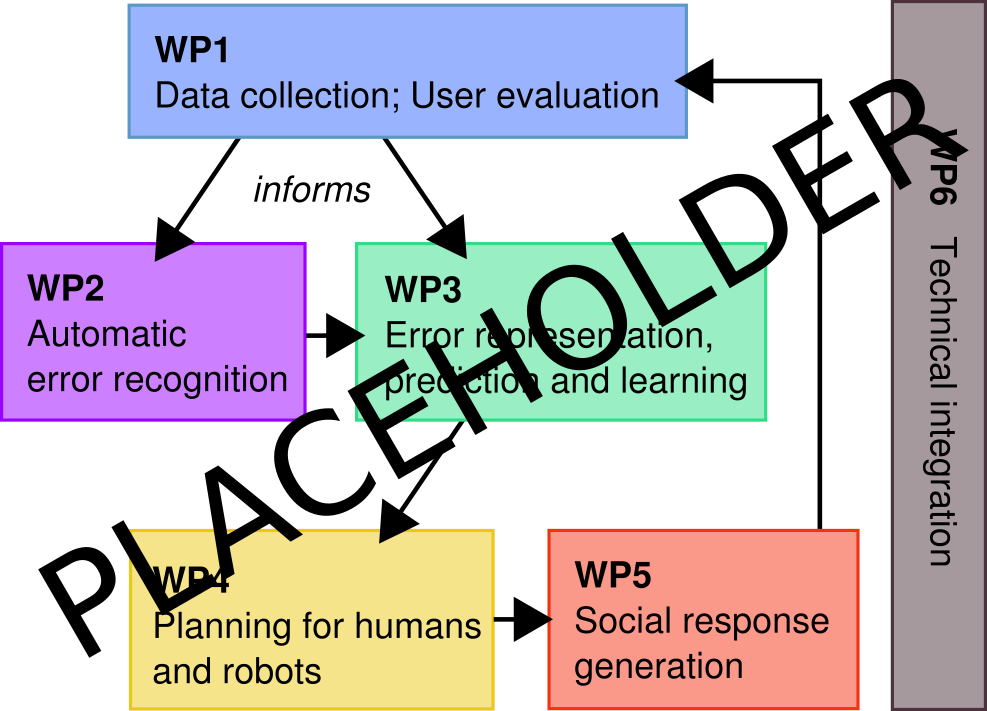
\includegraphics[width=0.8\linewidth]{figs/wp-interrelations}
    \caption{Inter-dependencies between work packages and main tasks}
    \label{}
\end{figure}



\section{Management structure, milestones and procedures}\label{management-structure-milestones-and-procedures}

\subsection{Milestones}\label{milestones}

\begin{itemize}

\item   week-long tests with local children in local schools
\item   field deployment with one child in one school
\end{itemize}

\begin{table}[!htbp]
\caption{List of milestones}
\centering
\begin{tabular}{@{}lllll@{}}
\toprule
\textbf{Milestone number} & \textbf{Milestone name} & \textbf{Related work package(s)} & \textbf{Estimated date} & \textbf{Means of verification} \\ \midrule
                          &                         &                                  &                         &                                \\
                          &                         &                                  &                         &                                \\
                          &                         &                                  &                         &                                \\
                          &                         &                                  &                         &                                \\ \bottomrule
\end{tabular}
\end{table}


\subsection{Risks}\label{risks}

\begin{table}[!htbp]
\caption{Identified risks and proposed mitigations}
\centering
\begin{tabular}{@{}lll@{}}
\toprule
\textbf{Description of risk} & \textbf{Work package(s) involved} & \textbf{Proposed risk mitigation measures} \\ \midrule
risk 1 (low/medium/high)     &                                   &                                            \\
                             &                                   &                                            \\
                             &                                   &                                            \\
                             &                                   &                                            \\ \bottomrule
\end{tabular}
\end{table}





\begin{itemize}
    \item week-long tests with local children in local schools
    \item field deployment with one child in one school
\end{itemize}


Plan to hire one mechatronics engineer and one interaction designer

Role of the mechatronics engineer: develop a novel platform, including -
chassis - power autonomy for one day - on-board compute suitable for
deep learning (NVidia TX2?) - vision (embedded RGB-D camera) - audio
processing

Role of the interaction designer: refine interaction modalities (in
particular, the non-verbal speech), details cross-modal interactions,
define interaction patterns with the child




\section{Measures for achieving impact}

\subsection{Dissemination and exploitation of results}

\subsection{Communication activities}

%%%%%%%%%%%%%%%%%%%%%%%%%%%%%%%%%%%%%%%%%%%%%%%%%%%%%%%%%%%%%%%%%%%%%%%%%%%%%%%%%%%%%%%%
%%%%%%%%%%%%%%%%%%%%%%%%%%%%%%%%%%%%%%%%%%%%%%%%%%%%%%%%%%%%%%%%%%%%%%%%%%%%%%%%%%%%%%%%
%%%%%%%%%%%%%%%%%%%%%%%%%%%%%%%%%%%%%%%%%%%%%%%%%%%%%%%%%%%%%%%%%%%%%%%%%%%%%%%%%%%%%%%%


\hypertarget{risk-assessment}{%
\subsubsection{Risk assessment}\label{risk-assessment}}

\hypertarget{c.-resources}{%
\subsection{c. Resources}\label{c.-resources}}


The \project project sets an ambitious target in term of technical development.
The project indeed requires unique technical skills, both software and
hardware-wise, to create, design and build the envisioned robotic systems.

Software-wise, PI Lemaignan is a leading
developer of software for intelligent robots, with numerous contributions to
the major software platforms used in robotic (including major contributions to
ROS, OpenCV, authoring of widely-used pieces of software like the ROS-naoqi
bridge used by hundred of researchers using the Nao and Pepper robots or the
MORSE robotic simulator). He has been teaching various modules related to
software development for robotics, and the breadth and depth of his knowledge of
robotic software development is well established. He will be leading the
software development, and, as part of the fellowship, he will also seek for
additional expert knowledge on (1) interaction design and (2) low-level
micro-programming to complete the set of required programming needs.

Hardware-wise, the Bristol Robotics Lab, where this fellowship will take place,
offer unique support and facilities for robotic hardware development: the
laboratory's dedicated equipment includes two industrial-grade rapid prototyping
machine, a laser cutter, one 5-axis digital milling machine, all the required
facilities for PCB prototyping, and a team of six full-time technicians,
specialised in hardware development. The BRL has indeed a long track-record of
designing and building new and original robots (from the BERT humanoid in the
FP7 CHRIS project, to micro-robotics [in...?], to [...]). \project will directly
benefit of this expertise, which will ensure a feasible and realistic technical
implementation of the \project robots. Besides, an hardware engineer, dedicated
to the project, will be recruited in the frame of the project.

The BRL also include a hardware incubator and is co-located with 70 start-ups
and SMEs specialising in robotic hardware and mechatronics (Bristol's
\emph{FutureSpace}). This combination of excellent research and vast industry
expertise on one site is unique in the UK, and is will play an instrumental role
in providing a coherent and strong pathway to impact to the project, including
further engagement with industrial partners and spin-off opportunities.


\hypertarget{host-institution}{%
\subsubsection{Host institution}\label{host-institution}}

The \emph{Bristol Robotics Laboratory (BRL)} is the largest co-located
and most comprehensive advanced robotics research establishment in the
UK. It is a joint venture between the University of the West of England
and the University of Bristol. BRL's multidisciplinary approach aims to
create autonomous devices capable of working independently, with each
other, or with humans. BRL draws on robotics, electrical \& mechanical
engineering, computer science, psychology, cognitive science and
sociology. BRL has an international reputation as a leading research
centre in advanced robotics research and has over 250 researchers
working on a broad portfolio of topics: HRI, collective robotics, aerial
robotics, neuro-inspired control, haptics, control systems, energy
harvesting and self-sustaining systems, rehabilitation robotics, soft
robotics and biomedical systems. BRL has many collaboration
partnerships, both national and international, and is experienced in
managing large multi-site projects. BRL has support from two embedded
units specialising in business and enterprise, together with an
incubator and successful track record of spin-outs.

\newpage

\printbibliography
\end{document}
